\documentclass[aps, amsmath, amssymb, nofootinbib, superscriptaddress, longbibliography, floatfix, eqsecnum, rmp, twocolumn]{revtex4-2}

\usepackage[pdftex]{graphicx}
\usepackage{mathrsfs}
\usepackage{amsmath}
\usepackage[colorlinks, breaklinks, urlcolor={blue}, linkcolor={red}, citecolor={blue}]{hyperref}
\usepackage{mathtools}
\usepackage[english]{babel}
\usepackage{booktabs}
\usepackage{type1cm}
\usepackage{caption}
\usepackage{subcaption}
\usepackage{url}
\usepackage{braket}
\usepackage{algorithm}
\usepackage{algpseudocodex}
\usepackage[strict]{changepage}
\usepackage{tikz}
\usepackage{tikz-3dplot}
\usepackage{pgfplots}
\usepackage{wasysym}
\usepackage{multirow}

\pgfplotsset{compat=newest}

\usetikzlibrary{positioning, fit, calc, shadows, shadows.blur, arrows.meta, shapes.geometric, fillbetween, fadings, quantikz2}

\let\oldalgorithmic\algorithmic
\let\endoldalgorithmic\endalgorithmic
\renewenvironment{algorithmic}
{\begin{adjustwidth}{-1em}{}\oldalgorithmic}
{\endoldalgorithmic\end{adjustwidth}}

\colorlet{nodeVLineColor}{blue}
\colorlet{nodeVFillColor}{cyan!20}
\colorlet{nodeULineColor}{orange}
\colorlet{nodeUFillColor}{yellow!20}
\colorlet{nodeRedLineColor}{red}
\colorlet{nodeRedFillColor}{red!20}
\colorlet{nodeGreenLineColor}{green}
\colorlet{nodeGreenFillColor}{green!20}
\colorlet{nodeBlueLineColor}{blue}
\colorlet{nodeBlueFillColor}{cyan!20}
\colorlet{nodeBlueLineColor}{blue}
\colorlet{nodeBlueFillColor}{cyan!20}
\colorlet{graphEdgeColor}{gray}
\colorlet{graphNonEdgeColor}{lightgray}
\colorlet{setDFillColor}{red!20}
\colorlet{setHFillColor}{green!20}
\colorlet{setHDFillColor}{blue!20}
\colorlet{topologyFillColor}{cyan!10}
\colorlet{blockchainDiscColor}{blue!10}
\colorlet{blockchainPendingDiscColor}{red!10}
\colorlet{redHighlightColor}{red!80}
\colorlet{blueHighlightColor}{blue!80}

\tikzset{
	genericStyle/.style = {
		every node/.style = {circle, draw, minimum size=2em}, >=latex
	}
}

\tikzset{
	myShadow/.style = {
		blur shadow = {shadow blur steps=5, shadow xshift=0.15em, shadow yshift=-0.1em}
	}
}

\tikzset{
	myLightShadow/.style = {
		blur shadow = {shadow blur steps=5, shadow xshift=0.1em, shadow yshift=-0.066em}
	}
}

\tikzset{
	nodeUStyle/.style = {
		draw=nodeULineColor, fill=nodeUFillColor, myShadow
	}
}

\tikzset{
	nodeVStyle/.style = {
		draw=nodeVLineColor, fill=nodeVFillColor, myShadow
	}
}

\tikzset{
	nodeGrayStyleC/.style = {
		draw=gray, fill=gray!20, myShadow
	}
}

\tikzset{
	nodeGrayStyle/.style = {
		draw=black, fill=gray!20, myShadow
	}
}

\tikzset{
	nodeLightGrayStyle/.style = {
		draw=gray, fill=lightgray!20, myShadow
	}
}

\tikzset{
	nodeRedStyle/.style = {
		draw=nodeRedLineColor, line width=0.25, line cap=round, fill=nodeRedFillColor, myLightShadow
	}
}

\tikzset{
	nodeBlueStyle/.style = {
		draw=nodeBlueLineColor, line width=0.25, line cap=round, fill=nodeBlueFillColor
	}
}

\tikzset{
	graphEdgeStyle/.style = {
		draw=graphEdgeColor, line width=1, line cap=round
	}
}
	
\tikzset{
	graphNonEdgeStyle/.style = {
		draw=graphNonEdgeColor, opacity=0.25, line width=1, line cap=round
	}
}

\tikzset{
	graphRedEdgeStyle/.style = {
		draw=red, opacity=0.5, line width=1.5, line cap=round
	}
}

\tikzset{
	graphLightRedEdgeStyle/.style = {
		draw=nodeRedLineColor, opacity=0.15
	}
}

\tikzset{
	graphBlueEdgeStyle/.style = {draw=blue!50, line width=0.5}
}

\frenchspacing
    
\captionsetup[figure]{margin=0pt, font=small, labelfont=bf, labelsep=endash, justification=centerlast, labelsep=colon}
\captionsetup[algorithm]{margin=0pt, font=small, labelfont=bf, labelsep=endash, justification=centerlast, labelsep=colon}
\usepackage{pifont}% http://ctan.org/pkg/pifont
\newcommand{\cmark}{\ding{51}}%
\newcommand{\xmark}{\ding{55}}%

\newcommand{\peter}[1]{\textcolor{red}{#1}}

\newtheorem{thm}{Theorem}%[section]
\newtheorem{prop}[thm]{Proposition}
\newtheorem{lem}[thm]{Lemma}
\newtheorem{rem}[thm]{Remark}
\newtheorem{defn}[thm]{Definition}

\begin{document}

\title{Review on IPQ-LWE-TCFs}

%\author{Peter P. Rohde}
\email[]{dr.rohde@gmail.com}
\homepage{http://www.peterrohde.org}
\affiliation{\mbox{BTQ Technologies, 16-104 555 Burrard Street, Vancouver BC, V7X 1M8 Canada}}
\affiliation{\mbox{Center for Engineered Quantum Systems, School of Mathematical \& Physical Sciences}, \mbox{Macquarie University, NSW 2109, Australia}}
\affiliation{\mbox{Hearne Institute for Theoretical Physics, Department of Physics \& Astronomy}, \mbox{Louisiana State University, Baton Rouge LA, United States}}


\date{\today}

\frenchspacing

\begin{abstract}
Quantum technology has major implications for information security, both in terms of code-breaking and -making, and the strategic interplay between the two. However these implications are far more nuanced than is often captured in the popular press. Here we provide a broad overview of different aspects of information security in the quantum era, examining the security implications of quantum technology and important long-term strategic considerations. This work is written at a non-expert level, providing an accessible overview where the limited amount of mathematics employed can safely be glossed over by the non-expert.
\end{abstract}

\maketitle

\tableofcontents
\section{Introduction} \label{introduction}

The implications of quantum technology for information security attracts a lot of attention in the popular press. But reading headline articles one could be forgiven for taking away something to the effect of,
\begin{quote}
	``Quantum computers will break all our present-day encryption, but quantum cryptography will save the day.''
\end{quote}
Both of these statements are false and there is far more nuance to the intersection between quantum technology and information security than what is often captured in the mainstream media. Here we'd like to give a more detailed overview of what this intersection looks like and how, in our minds, things are likely to play out.

We'll approach this by looking at both classical and quantum cryptographic protocols, their various nuances and caveats, what their different vulnerabilities are, and what implications this has both presently and in the future.

\subsection{What is security?} \label{what-is-security}

When cryptographers talk about security there are different standards of security they have in mind:
\begin{itemize}
	\item \emph{Computational security} is security based on the assumption that adversaries do not possess sufficient computational power to crack our encryption and haven't made any major algorithmic developments that might reduce the computational power they need.
	\item \emph{Information-theoretic security} refers to the situation where a cryptographic system can be mathematically proven to offer perfect security in the absence of any assumptions about computational power.
\end{itemize}

The second standard sets a much higher bar than the former. But because this bar is so high it is often not possible to find cryptographic systems that have this property. When we hear in the media how quantum computers have the potential to break certain cryptographic codes, this is because those codes have relied on the computational security assumption which would not hold were quantum computers available.

If a protocol can be proven to be information-theoretically secure, we're in business and have little to worry about. However very few protocols exhibit this property, and in the classical case, there is only one known example, the one-time-pad, or Vernam cipher (Sec.~\ref{one-time-pad-encryption}), which has extremely limited utility.

In the case of computational security, things are more nuanced, since there are different types of physically realisable computers: quantum and classical. To consider this more rigorously we need to turn to the field of \emph{computational complexity theory} \cite{bib:arora2009computational}, which studies what classes of problems can be solved by different computational models, giving rise to \emph{complexity classes}. There are countless such complexity classes \cite{bib:ComplexityZoo}. Some of these correspond to physically realisable computational models, while others are not physically realisable but useful mathematical tools for use in derivations and proofs. Here we will focus on just a few of these:
\begin{itemize}
	\item \textbf{P} denotes the class of problems that can be solved in polynomial time (as a function of problem size) on a classical computer. These problems are regarded as \emph{classically efficient} by computer scientists.
	\item \textbf{BPP} is the same as \textbf{P} but the computer has access to a random number generator and is able to operate probabilistically. It is known that $\mathbf{P}\subseteq\mathbf{BPP}$ but unproven whether $\mathbf{P}=\mathbf{BPP}$.
	\item \textbf{NP} denotes the class of problems that can be verified (but not necessarily solved) in polynomial time on a classical computer. It is known that \mbox{$\mathbf{P}\subseteq\mathbf{NP}$} and believed but not proven that \mbox{$\mathbf{P}\subset\mathbf{NP}$}. %Whether \mbox{$\mathbf{P}=\mathbf{NP}$} is one of the great open problems in computer science.
	\item \textbf{BQP} denotes the class of problems that can be solved on a quantum computer in polynomial time (i.e efficient for quantum computers). It is known that \mbox{$\mathbf{BPP}\subseteq\mathbf{BQP}$} and believed but not proven that \mbox{$\mathbf{BPP}\subset\mathbf{BQP}$}. If the latter were not the case, there would be no exponential advantage offered by quantum computers over classical ones.
	\item Everything outside \textbf{BPP} and \textbf{BQP} cannot be efficiently solved on any physically realisable computational device (assuming there aren't any laws of physics beyond quantum physics, which is also just a strongly held assumption). \textbf{NP} is an example of a complexity class not believed to be physically realisable.
\end{itemize}

Fig.~\ref{fig:complexity} illustrates the believed relationships between these classes as a Venn diagram, also showing where some classes of cryptographic algorithms belong.

\begin{figure}[!htb]
	\centering
	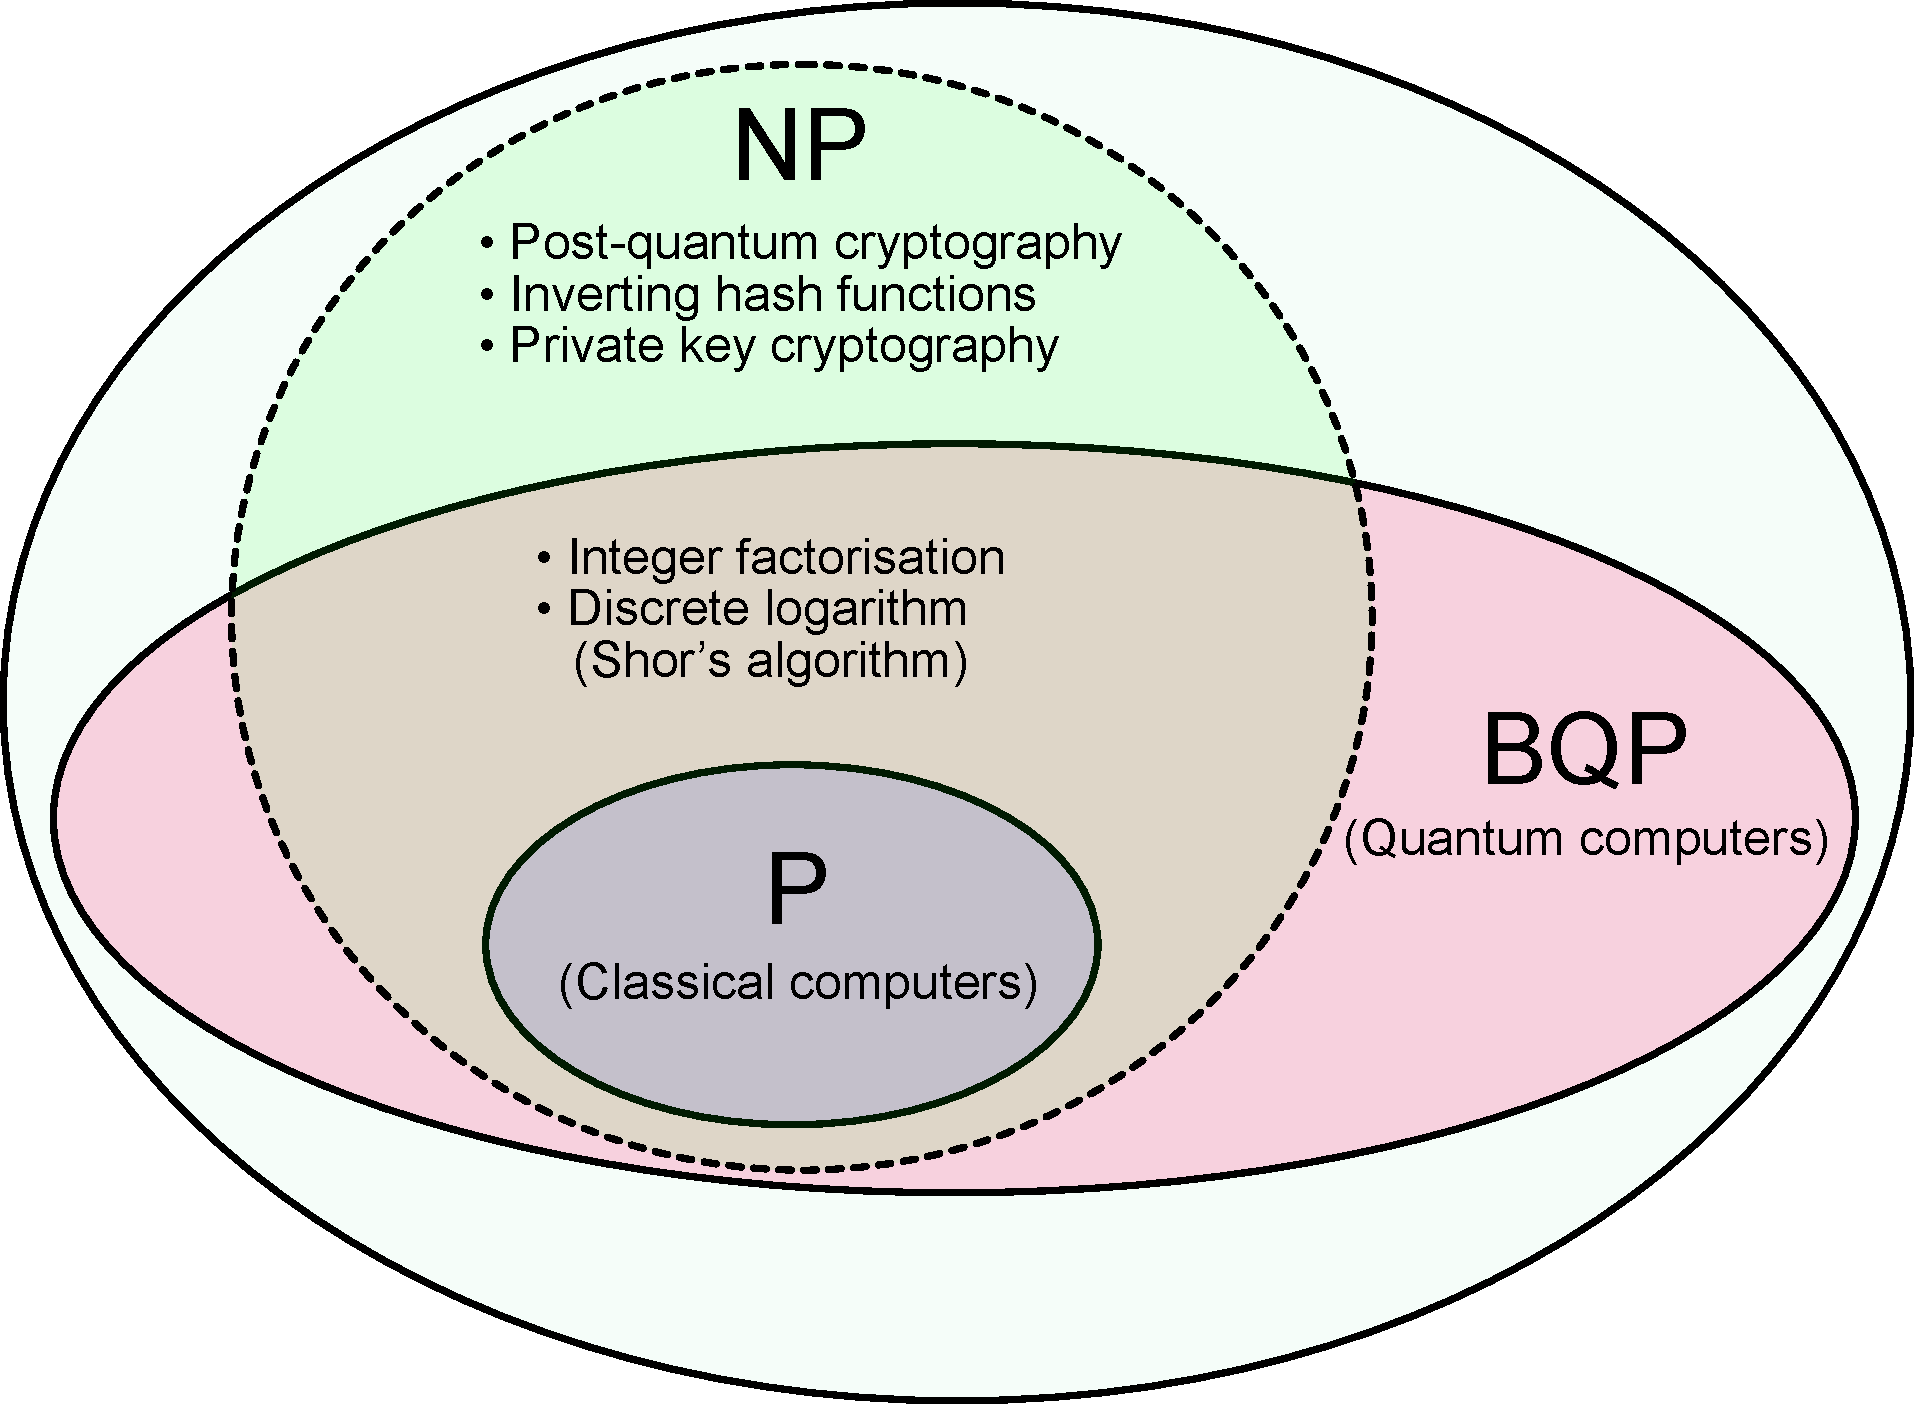
\includegraphics[width=\columnwidth]{figures/Complexity_classes}
	\caption{Venn diagram of the believed relationships between some complexity classes relevant to classical and quantum computing and cryptography. \textbf{P} is the class of problems that can be efficiently solved on a classical computer. \textbf{BQP} is the same for quantum computers. Problems outside \textbf{P} and \textbf{BQP} cannot be efficiently solved by any physically realisable computer (unless the laws of quantum physics are incorrect). Since $\mathbf{P}\subseteq\mathbf{BQP}$, quantum computers can efficiently solve classical problems, but the converse is not believed to be true since it is believed but not proven that $\mathbf{P}\subset\mathbf{BQP}$. \textbf{NP} is the class of problems that can be efficiently verified (as opposed to solved) on a classical computer. While \textbf{P} and \textbf{BQP} are physically realisable computational models, \textbf{NP} is not believed to be, instead being a theoretical one. In general, breaking crypto-systems resides in \textbf{NP} since this can be efficiently verified but not efficiently solved.} \label{fig:complexity}
\end{figure}

If a cryptographic problem is known to reside in \textbf{BQP} but not in \textbf{P}, it can be compromised by quantum computers but not by classical computers. This is where we believe the integer factorisation and discrete logarithm problems reside, which form the basis of current public-key cryptography. Note that neither of these problems has been \emph{proven} to lie outside of \textbf{P} --- it is a strongly held belief based on the fact that these problems have been incredibly well studied. But who knows, perhaps we just haven't studied them hard enough?

For \emph{post-quantum cryptography} (Sec.~\ref{post-quantum-cryptography-pqc}) the ultimate goal is to develop protocols whereby decryption in the absence of knowing the key provably lies outside of \textbf{BQP}. However the field of computational complexity is an extremely challenging one, and many very basic identities are assumed to hold, but not proven to. The most famous example of this is the \textbf{P} versus \textbf{NP} problem, a thorn in the side of computer scientists for decades. Roughly speaking, this statement asks ``if a problem is easy to verify is it easy to solve?'', the answer to which is understood but not proven to be ``no''. The difficulty in proving these complexity relationships often means we have to accept weaker computational security assumptions.
\section{Quantum computing and communications} \label{quantum_computing}
\subsection{Quantum states}

In quantum mechanics, a \textit{quantum state} is a unit vector in the complex space $\mathbb{C}^N$.
As in classical computing, all computations are performed using classical bits, $0$ and $1$. In quantum computing, we use an equivalent term that has more interesting properties: the \textit{quantum bit} or \textit{qubit}. A qubit, a two-level system, can be considered the simplest unit of quantum information. Let us use Dirac notation and denote $\ket{0}$ and $\ket{1}$ as the two basis states of a qubit, similar to the classical case. The $\ket{0}$ and $\ket{1}$ are called `kets', more explanation about the use of this notation will be proposed soon in this section.

The first special property of a quantum state is \textit{superposition}, where a quantum system is not necessarily in one specific state but can be in a \textit{superposition} of them. Hence, a quantum state $\ket{\psi}$ can be expressed as a linear combination of the two basis states $\ket{0}$ and $\ket{1}$,
\begin{align}
\ket{\psi}=\alpha\ket{0}+\beta\ket{1}.
\label{eq:quantumstate}
\end{align}
Note that the coefficients $\alpha$ and $\beta$ are complex numbers called amplitudes. They represent the probability amplitudes of getting the results $0$ and $1$ if one measures the state. We have that
\begin{align}
\Pr[0] &= |\alpha|^2,\nonumber\\
\Pr[1] &= |\beta|^2,\nonumber\\
|\alpha|^2 + |\beta|^2 &= 1.
\end{align}

One simple example is that if one has the 
%Write about the + and - states

This ``weird'' property of qubits makes the idea of quantum computers more promising since with $n$ classical bits, one can perform up to $n$ computations, while with $n$ qubits, this number could reach up to $2^n$ computations \peter{Not computations, rather terms in the superposition}.

\noindent Recall that quantum states can be written as vectors in complex space; hence, using the Dirac notation for describing quantum states simplifies linear algebra operations while working with these states. Note that kets are column vectors, for example:
\begin{align}
    \ket{0}=\begin{bmatrix} 1\\ 0
\end{bmatrix} \text{, }\ket{1}=\begin{bmatrix} 0\\1
\end{bmatrix}
\end{align}
The superposition state~\eqref{eq:quantumstate} can be represented as the following vector:
\begin{align}
    \ket{\psi}=\alpha\ket{0}+\beta\ket{1} = \begin{bmatrix} \alpha\\ \beta
\end{bmatrix}.
\end{align}

Working with row vectors in complex vector space, we also need to deal with \textit{conjugate transpose}, ie. row vectors. In the Dirac notation, these row vectors are called ``bras'', for example
\begin{align}
    \bra{0}= \begin{bmatrix} 1 & 0 \end{bmatrix} \text{, }\bra{1}=\begin{bmatrix} 0 & 1
\end{bmatrix},
\end{align}
and 
\begin{align}
    \bra{\psi}=  \begin{bmatrix} \alpha^* & \beta^*\end{bmatrix}
\end{align}
where $\alpha^*$ and $\beta^*$ are complex conjugates of $\alpha$ and $\beta$.

%The pair $\{\ket{0},\ket{1}\}$ are orthogonal and is called 

\subsection{Measurement basis}

\subsection{No-cloning theorem}
\section{Lattice-based post-quantum cryptography} \label{post-quantum-cryptography-pqc}

\subsection{Lattices}
\subsubsection{Definitions}\label{lattice}
\begin{defn}
    Lattices in $\mathbb{R}^n$ are discrete subgroup of $\mathbb{R}^n$. Consider integer lattice $\mathcal{L}\subseteq \mathbb{Z}^n$, $\mathcal{L}$ can be represented by a basis $\mathbf{B}=[\mathbf{b}_1,\cdots,\mathbf{b}_n]\in\mathbb{Z}^{m\times n}$, where each vector $\mathbf{b}_i$ is written in column form as follow: 

$$\mathcal{L}(\mathbf{B}):=\left\{\sum_{i=1}^n\mathbf{b}_i x_i | x_i\in\mathbb{Z}~\forall i=1,\cdots,n \right\}\subseteq\mathbb{Z}^m.$$ 
\end{defn}

We refer to $n$ as the rank of the lattice $\mathcal{L}$ and $m$ as its dimension. $\mathcal{L}$ is called a full-rank lattice if $n=m$.

For a basis $\mathbf{B}$ of $\mathcal{L}$, we called $P(\mathbf{B})=\{\mathbf{B}\mathbf{x}|\mathbf{x}\in[0,1)^n\}$ is the fundamental parallelepiped of $\mathbf{B}$. A ``good'' basis of $\mathcal{L}$ results in a parallelepiped that is more square-like, whereas a ``bad'' basis produces a very thin parallelepiped. We denote$\|\mathbf{B}\|:=\max_{1 \le i \le k} \|\mathbf{b}_i\|$ the maximum $l_2$ length of the vectors in $\mathbf{B}$ and $\tilde{\mathbf{B}}:=\{\tilde{\mathbf{b}}_1,\cdots,\tilde{\mathbf{b}}_k \}$ the Gram-Schmidt orthogonalization of the vectors $\mathbf{b}_1,\cdots,\mathbf{b}_k$ in that order.


\begin{figure}[!htb]
	\centering
	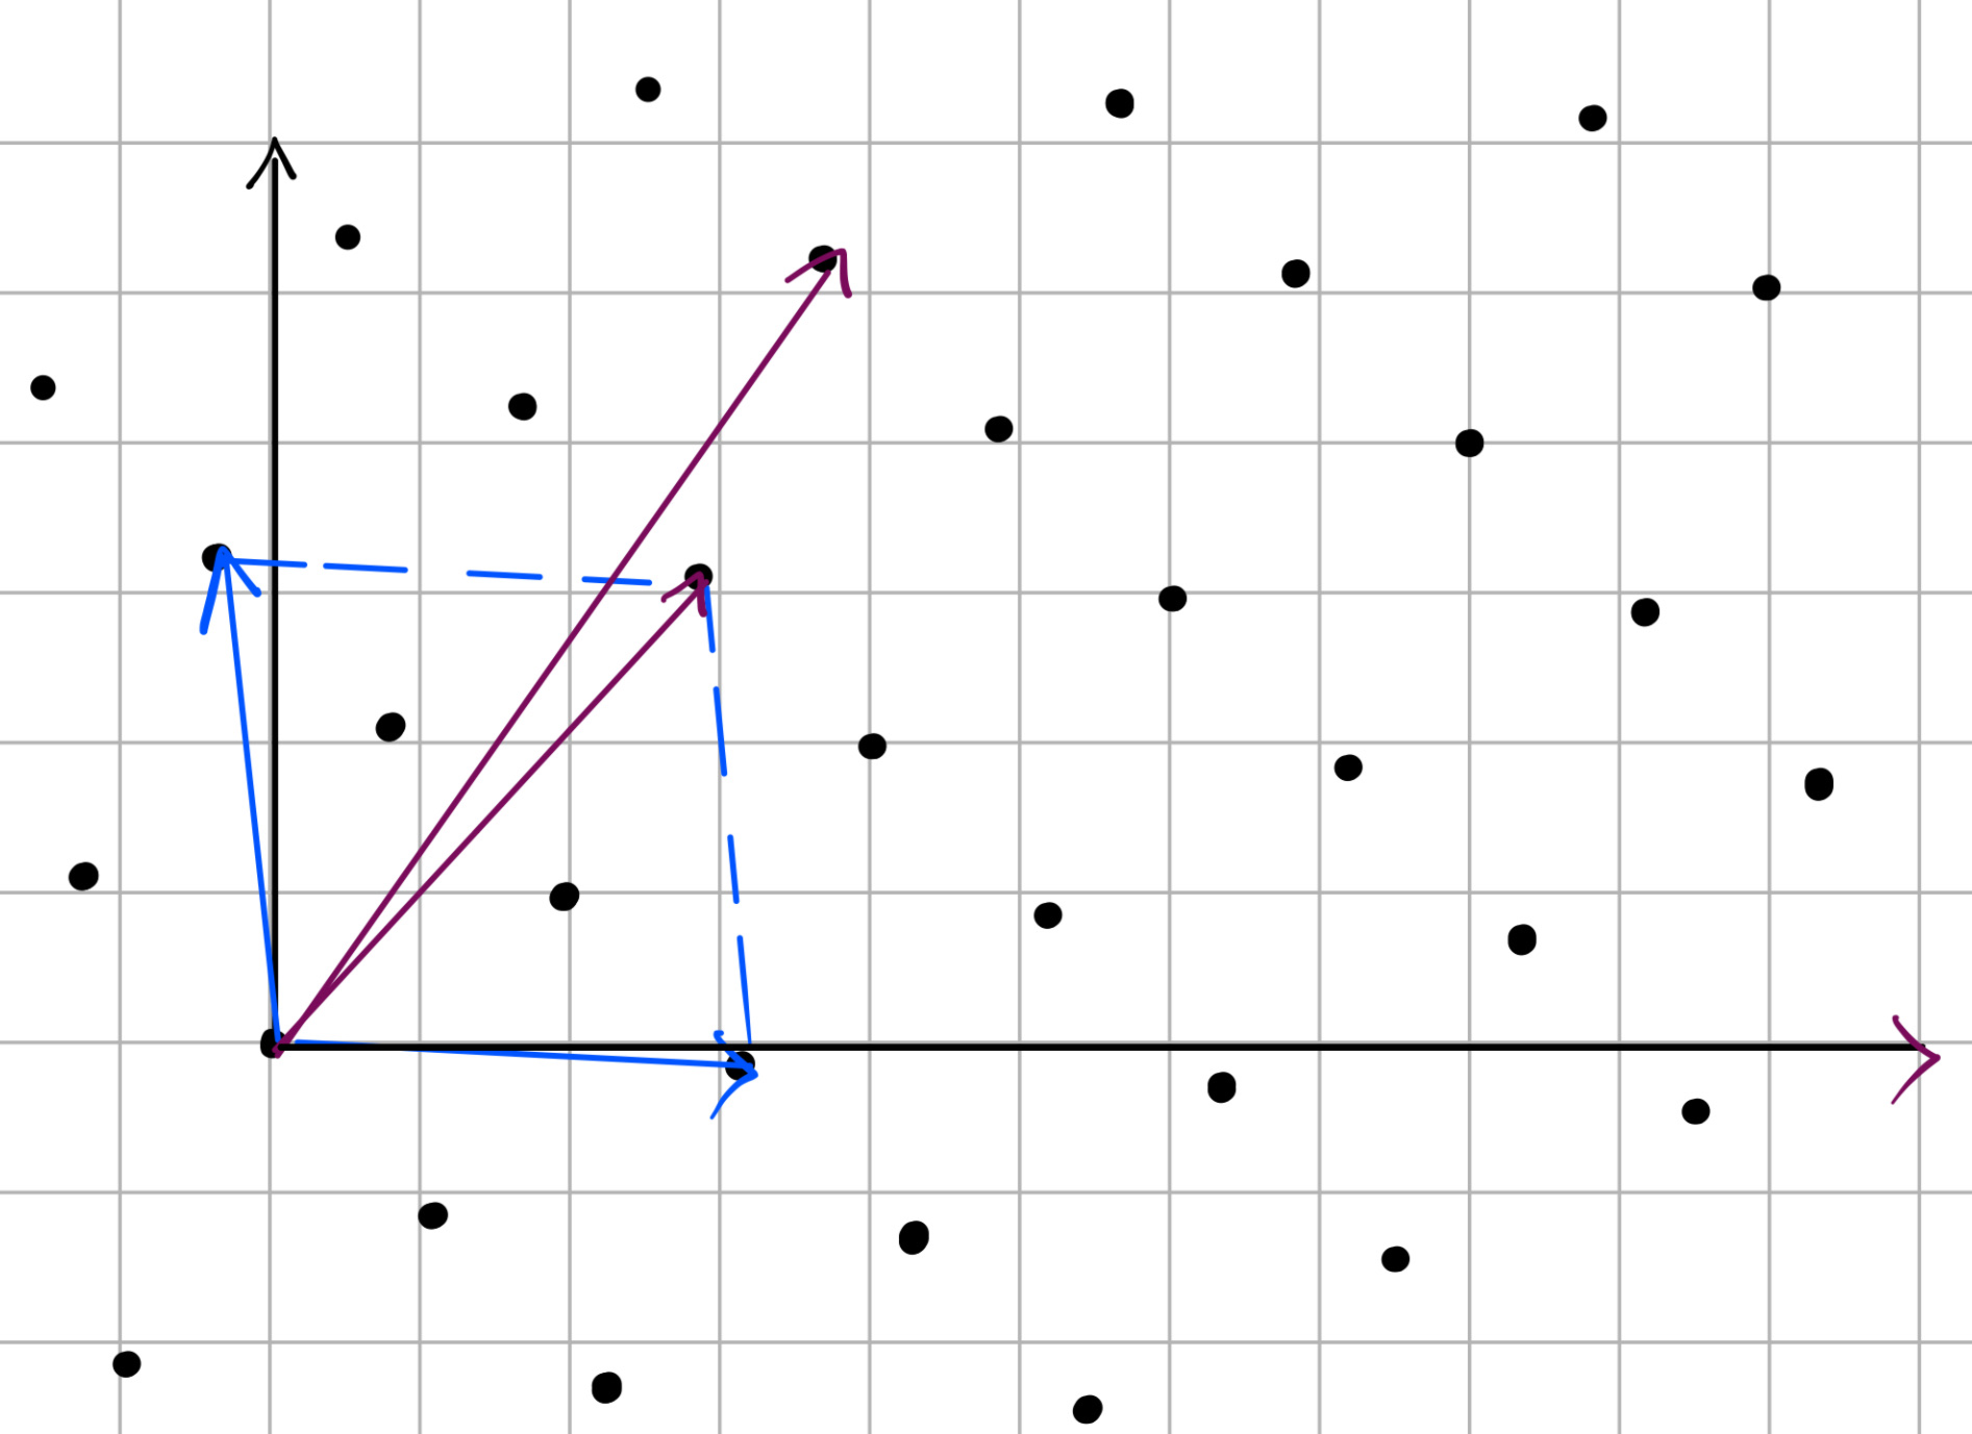
\includegraphics[scale=0.3]{figures/lattice_basis.pdf}
	\caption{Consider a two-dimensional lattice $\mathcal{L}$,  a basis for $\mathcal{L}$ consists of two non-zero vectors  $u$ and  $v$ such that any vector in $\mathcal{L}$ can be written as a linear combination of $u$ and $v$. A good basis for $\mathcal{L}$ will have vectors with lengths that are close to each other and an angle between them that is close to $90$ degrees.}\label{fig:lattice_basis}
\end{figure}

%\subsubsection{Hardness assumptions}

For a given lattice $\mathcal{L}(\mathbf{A})$, one basic parameter is the length of the shortest vector $\mathbf{s}$, denoted as $\lambda_1 = \|\mathbf{s}\|$ \peter{Here we should first define what \textbf{s} is}. This parameter is also called \textit{successive minima} if one considers the scenario where $\lambda_1$ is the smallest $r$ such that all the lattice points inside a ball of radius $r$ $\overline{\mathcal{B}}(0,r)$ span a space of dimension $1$. Similarly, we can define the $n^{th}$ successive minimum of $\mathcal{L}(\mathbf{A})$ as $\lambda_n(\mathcal{L}) = \inf\{r|\dim(\mathsf{span}(\mathcal{L}\cap \overline{\mathcal{B}}(0,r)))\leq n\}$.

%\textcolor{red}{Add an figure of sucessive minimum}

Hence, one of the most important problems in lattice-based cryptography is the Shortest Vector Problem ($\mathsf{SVP}$), which asks to find the shortest nonzero vector $\mathbf{s}$ in a given lattice $\mathcal{L}(\mathbf{A})$ with an arbitrary basis $\mathbf{A}$. There are also approximate versions of this problem called $\mathsf{SVP}_{\gamma}$ where the goal is to find a nonzero vector that is of length at most $\gamma = \gamma(n)\geq 1$ times the length of the optimal solution.

The ``decision'' versions of the problem ask to determine whether a given number $d$ is the minimum distance of $\mathcal{L}(\mathbf{A})$, i.e., $d = \min_{\mathbf{0}\neq \mathbf{v}\in\mathcal{L}}\|\mathbf{v}\|$.
This problem is known to be NP-hard in the $\ell_{\infty}$ norm, meaning there is no known polynomial-time algorithm to solve it~\cite{hardness_of_SVP}. For the $\ell_2$ (Euclid) norm, it remains a long-standing open problem. Another important problem is the Shortest Independent Vectors Problem ($\mathsf{SIVP}_{\gamma}$) with an approximation factor $\gamma$, a given a lattice $\mathcal{L}(\mathbf{A})$ with an arbitrary basis $\mathbf{A}$, $\mathsf{SIVP}_{\gamma}$ asks to find find $n$ linearly independent lattice vectors of length at most $\gamma(n)\cdot \lambda_{n}(\mathcal{L})$ where $\lambda_{n}(\mathcal{L})$ is the $n^{th}$ successive minimum of $\mathcal{L}$. Like $\mathsf{SVP}$, $\mathsf{SIVP}$ is also NP-hard.

\noindent Many hardness problems in lattice-based cryptography can be \textbf{``reduced''} to instances of $\mathsf{SVP}$ or $\mathsf{SIVP}$, for more information about reductions between lattice problems, please refer to~\ref{reduction} and ~\cite{reduction_lattice}.

\peter{The above intro on lattices we might expand upon to make it more accessible to a non-specialist audience.}

\subsubsection{Reductions}\label{reduction}

Within the realm of computational hardness challenges, the term ``reduction'' denotes a methodological approach whereby one problem is transformed into another, such that solving the second problem enables solving the first. This is a formal way to compare the intrinsic difficulty of different problems.  Specifically, if problem A can be reduced to problem B, and if one has a solution to B, then A can be solved. This doesn't necessarily imply that A is as hard as B, but that B is at least as hard as A. 

In the analysis of problem hardness, distinctions are made between \textit{worst-case} and \textit{average-case} scenarios. The \textit{worst-case} scenario is the most difficult possible instance for a given problem while the \textit{average-case} looks at the expected performance of an algorithm across all possible instances of a problem, usually under some reasonable assumption about the distribution of these instances. 

In Post-Quantum Cryptography (PQC), reductions are the main technique used to prove the security of cryptographic protocols by reducing their hardness to well-known hard problems. If such a reduction exists, then finding an efficient way to break the system would imply an efficient solution to the underlying hard problem, which is presumed not to exist, thus the security of the protocol holds.

%\textcolor{red}{Add an figure of reduction!!!!!! Can we illustrate reduction using some diagram?}


\subsection{SIS and LWE problems}
Let us first consider solving the linear equation
\begin{align}
    \mathbf{A}\mathbf{s} = \mathbf{y}\mod q \label{eq:linear_equation}
\end{align}

given $n,m \in \mathbb{Z}$, a prime number $q$, a matrix $\mathbf{A}$ in $\mathbb{Z}^{m\times n}_q$ and $\mathbf{y}$ is a vector in $\mathbb{Z}^m_q$. 

We can now view the matrix $\mathbf{A}$ as a basis for a lattice $\mathcal{L}(\mathbf{A})$. Note that solving Eq.~\eqref{eq:linear_equation} is achievable through Gaussian elimination. However, its variations, along with many other related lattice problems, are known to be NP-hard (based on the factors of polynomial approximation problems). Here, we highlight some significant lattice problems: \textbf{The shortest integer solution (SIS)} and \textbf{The Learning With Errors (LWE)} problems, further information on lattice-related problems can be found in~\cite{Pei16}.

\subsubsection{The shortest integer solution (SIS)}

Recall that initially, we are attempting to find a solution for the equation $\mathbf{A}\mathbf{s} = \mathbf{y} \mod q$. Consider an additional constraint that $\mathbf{s}$ is ``short'', i.e $\mathbf{s}$ lies in the subset $S=\{0,1\}^n\in\mathbb{Z}^n_q$; or more generally, $S=[-B,\dots, B]^n$  ($B\ll q/2$). Since we are seeking a \textit{short solution} to linear equations, this problem is referred to as the \textit{Short Integer Solution} (SIS) problem. Many cryptographic protocol deal with the case $\mathbf{y}=\mathbf{0}$, the $\mathbf{SIS}_{n,m,q,B}$ problem can be stated as follows:

\begin{defn}
    Let $n,m,q, B \in \mathbb{N}$ be positive integers. Given a uniformly sampled matrix $\mathbf{A}\in\mathbb{Z}^{n\times m}_q$, the shortest integer solution problem asks to find a none zero vector $\mathbf{s}\in\mathbb{Z}^m_q$ such that $\mathbf{A}\mathbf{s}=\mathbf{0}\mod q$ and $\|x\|_{\infty}\leq B$.
\end{defn}

One should think of $n$ as the security parameter that defines the hardness of the problem (the bigger $n$ is, the harder the problem becomes), $m$ usually depends on the specific application, generally $m\gg n$, $q=poly(n)$ and $B$ should be set large enough to ensure that a solution exists, but not trivial to solve. It is proven that solving the $\mathbf{SIS}_{n,m,q, B}$ problem is at least as hard as solving the $\mathsf{SVP}_{\gamma}$ on worst-case $n$-dimensional lattices with high probability for some approximation factor $\gamma$~\cite{Pei16}.


\subsubsection{The learning with errors problem (LWE)}
This subsection recalls the definition of the Learning With Errors (LWE) problem~\cite{Pei16}. Let's revisit Eq.~\eqref{eq:linear_equation}, we can consider a slight variant of it where the input pair $(\mathbf{A}\in \mathbb{Z}^{m\times n}_q, \mathbf{y} \in \mathbb{Z}^m)$ satisfies
\begin{align}
    \mathbf{A}\mathbf{s} + \mathbf{e}= \mathbf{y}\mod q \label{eq:lwe}
\end{align}
where $n, m, q$ are positive integers and $\mathbf{e}$ is an additional small noise term sample from an error distribution $\chi$ over $\mathbb{Z}^n$. 

The ``search'' $\mathsf{LWE}_{n,m,q,\chi}$ problem asks to find $\mathbf{s}\in\mathbb{Z}^n$ and the ``decision'' version asks to to distinguish between the distribution $ (\mathbf{A},\mathbf{y}=\mathbf{A}\mathbf{s}+\mathbf{e} \mod q)$ and a uniformly random sample $(\overline{\mathbf{A}},\mathbf{u})$.

The error term $\mathbf{e}$ effectively affects the exact relationship between the secret $\mathbf{s}$ and $\mathbf{y}$. Specifically, this term $\mathbf{e}$ ensures that although anyone can observe the pairs $(\mathbf{A},\mathbf{y})$, extracting the information of $\mathbf{s}$ is computationally infeasible if the problem is properly parameterized. The hardness of the $\mathsf{LWE}_{n,m,q,\chi}$ problem (and thus the security of many $\mathsf{LWE}$-based cryptosystems) relies on the assumption that finding $\mathbf{s}$ with random errors is as difficult as solving certain worst-case problems on lattices, more information is mentioned in~\ref{reduction}.

\subsubsection{Distribution over lattices}
It's important to note that the choice of the error distribution $\chi$ is crucial. A widely utilized distribution in numerous lattice-based cryptosystems is the Discrete Gaussian distribution. Typically, the discrete Gaussian is chosen in a way that ensures the errors $\mathbf{e}$ are small enough to allow for the correct extraction of the secret information but large enough to prevent adversaries from solving the problem.


For any positive integer $n$ and real $\sigma>0$, which is taken to be $1$ when omitted, the \textit{Gaussian function} $\rho_{\sigma}:\mathbb{R}^n\to \mathbb{R}^+$ of parameter (or width) $\sigma$ is defined 
\begin{align}
    \rho_{\sigma}(\mathbf{s}):=\exp(-\pi\|\mathbf{s}|\|^2/\sigma^2).
\end{align}

A \textbf{discrete Gaussian probability distribution} $D_{\mathcal{L},\sigma}$ over a lattice $\mathcal{L}$ is given by
\begin{align}
    D_{\mathcal{L},\sigma}(\mathbf{s})=\displaystyle{\frac{\rho_{\sigma}(\mathbf{s})}{\rho_{\sigma}{\mathcal{L}}}}, \forall \mathbf{s}\in\mathcal{L}.
\end{align}


The utilization of Gaussian distributions comes from its ability to effectively connect the Learning With Errors (LWE) problem to the worst-case scenario of the lattice NP-hard problems, thus providing a solid foundation for cryptographic security.

More concretely, a long sequence of works has established progressively stronger results about the worst-case lattice problems. It is shown that for any $\alpha>0$ such that $\sigma=\alpha q \geq 2\sqrt{n}$, the $\mathsf{LWE}_{n,m,q, D_{\mathbb{Z}_q,\sigma}}$, where $D_{\mathbb{Z}_q,\sigma}$ is the discrete Gaussian distribution, is at least as hard as approximating the shortest independent vector problem $(\mathsf{SIVP}_{\gamma})$ to within a factor of $\gamma = \Tilde{O}(n/\alpha)$~\cite{Reg09,RPS17}.

%For a lattice $\mathcal{L}$ and $\epsilon>0$, the smoothing parameter $\eta_{\epsilon}(\mathcal{L})$ of $\mathcal{L}$ is the smallest number $s$ satisfied $\rho_{1/\sigma}(\mathcal{L}^*\setminus \{0\})\leq \epsilon$.


%\begin{lem} For a lattice $\mathcal{L}$, a vector $\mathbf{c}\in\mathbb{R}^n$, $\epsilon>0$ and $\sigma\geq \eta_{\epsilon}(\mathcal{L})$, the statistical distance between $D_{\sigma}+\mathbf{c}\mod \mathcal{L}$ and the uniform distribution $\mathbb{R}^n/\mathcal{L}$ is at most $\epsilon/2$.\end{lem}


\subsubsection{Trapdoor mechanism}

In cryptography, a \textbf{trapdoor} refers to a concealed backdoor embedded within an algorithm or a specific piece of data. The idea is that, except for the individuals authorized to hold the trapdoor, others cannot extract any information about the trapdoor. This characteristic enables secure communication between parties. This subsection revisits certain trapdoor mechanisms to provide a fundamental understanding of the relationship between lattices and their trapdoors.

The first approach to constructing trapdoors for lattices involves the use of short bases, as these lead to more efficient algorithms for solving lattice problems. Algorithms designed to tackle challenges such as the Shortest Vector Problem (SVP) or the Closest Vector Problem (CVP) become more practical with basis vectors that are short and nearly orthogonal~\ref{lattice}. This is because the computations involved are simpler and can be executed more swiftly. Specifically, for solving the LWE problem using a short basis, one strategy employs Babai's nearest plane algorithm~\cite{Babai}. The initial step involves utilizing a short basis $\mathbf{T}_{\mathbf{A}}$ of a lattice $\mathcal{L}(\mathbf{A})$ to identify the lattice vector closest to $\mathbf{y}$. Given that the error is sufficiently ``small'', it becomes feasible to extract the secret vector $\mathbf{s}$'s information. A sequence of works has been carried out to develop more trapdoor mechanisms. Two of the notable approaches are~\cite{AP09} and~\cite{MP12}.

\cite{AP09} presented an algorithm to sample a uniform matrix $\mathbf{A}\in\mathbb{Z}_q^{n\times m}$ together with an associated basis $\mathbf{T}$ of $\mathcal{L}({\mathbf{A}})$ with a low Gram-Schmidt norm such that $\mathbf{A}\mathbf{T}_{\mathbf{A}} = \mathbf{0}$ as the public matrix and its secret trapdoor. The second approach is the trapdoor technique from~\cite{MP12}, which we focus on more due to its simpler, more elegant nature, and its support for more efficient cryptographic constructions.

\cite{MP12} first defined a ``primitive vector'' $\mathbf{g}=\{g_1,\dots,g_k\}\in\mathbb{Z}^k_q$ where $\gcd(g_1,\dots,g_k,q)=1$. Then
a matrix $\mathbf{G}\in\mathbb{Z}^{n\times m}_q$ is called ``primitive matrix'' if its columns generate all of $\mathbb{Z}^n_q$, i.e., $\mathbf{G}\mathbb{Z}^m=\mathbb{Z}^n_q$. We can now define the $\mathbf{G}$-trapdoor of a lattice $\mathcal{L}$ is a matrix $\mathbf{R}\in\mathbb{Z}^{(m-\omega)\times \omega}$ such that $\mathbf{A}\begin{pmatrix}
    \mathbf{R}\\ 
    \mathbf{I}
  \end{pmatrix} = \mathbf{H}\mathbf{G}$ for some invertible matrix $\mathbf{H}\in\mathbb{Z}^{n\times n}_q$. We refer to $\mathbf{H}$ as the \textbf{tag} or \textbf{label} of the trapdoor. 

The paper also presented an efficient algorithm $\mathsf{GenTrap}(1^n,1^m,q)$ that returns a matrix $\mathbf{A}\in\mathbb{Z}^{n\times m}_q$ and a trapdoor $\mathbf{T}_{\mathbf{A}}=\mathbf{R}$ such that the distribution of $\mathbf{A}$ is negligibly (in $n$) close to the uniform distribution. 

Moreover, there is an efficient algorithm $\mathsf{Invert}$ that, on input $\mathbf{A}$, $t_{\mathbf{A}}$ and $\mathbf{A}\mathbf{s}+\mathbf{y}$ where $\mathbf{s}\in\mathbb{Z}^n_q$ is arbitrary and $\mathbf{y}\gets \mathcal{D}_{\mathbb{Z}^m,\alpha q}$ for $1/\alpha \geq \sqrt{n\log q}\cdot \omega(\sqrt{\log n})$, outputs $\mathbf{s}$ and $\mathbf{y}$ with overwhelming probability over $(\mathbf{A},\mathbf{t}_{\mathbf{A}})\gets \mathsf{GenTrap}(1^n,1^m,q)$. By using the ``strong'' trapdoor $\mathbf{R}$, one also can efficiently generate the ``weak'' trapdoor $\mathbf{T}_{\mathbf{A}}$ or $\mathbf{s}$. Since in lattice-based PQC, these trapdoors $\mathbf{R},\mathbf{T}_{\mathbf{A}}, \mathbf{s}$ can be used as the secret keys of hierarchical parties in some hierarchical cryptosystems.

\peter{The above we could also expand to make more accessible.}

\subsection{RLWE problem}

There is a variant of the LWE problem that has been widely used in recent years called the Ring Learning With Error problem (RLWE). The primary benefit of using polynomial rings in RLWE offer more efficient and practical implementations of cryptographic schemes with significantly smaller keys and signature sizes while maintaining strong security guarantees.

Here, let's first recall some basic ideas of the RLWE problem.

\subsubsection{The initial idea.}
Let's recall that the SIS problem in Eq.~\eqref{eq:linear_equation} yields a very simple collision-resistant hash function that is provably secure if worst-case lattice problems are hard:
\begin{align}
    h_{\mathbf{A}}(\mathbf{s})=\mathbf{A}\mathbf{s} \mod q
\end{align}
where $\mathbf{A}\in\mathbb{Z}^{m\times n}_q$ is uniformly random and $\mathbf{s}\in \{0,1\}^n$. 

However, this is inefficient, since just reading the public description of $\mathbf{A}$ takes time roughly $mn\log q>n^2$. The goal is now to show a variant of $h_{\mathbf{A}}$ whose running time is roughly linear in $n$. 

A trivial idea is taking some short, uniformly random seed $r$ and then setting $\mathbf{A} = H(\textsf{seed})$ for some suitable expanding function $H$. However, we need to describe $H$ so that it can be efficiently used in cryptography constructions. 


Let's first take the random seed to be $\ell = m/n$ uniformly random vectors $\mathbf{a}_1,\dots,\bf{a_{\ell}}\in[q]^n$. Consider the ``cyclic rotations'' of $\mathbf{a}_i$, i.e. for a single vector $\mathbf{a}=(a_1,\dots,a_n)^T\in\mathbb{Z}^n$, we define
\begin{align}
    \mathsf{Rot}(\mathbf{a})=
    \begin{pmatrix}
    a_1 & a_n &\dots& a_3 & a_2\\
    a_2 & a_n &\dots& a_4 & a_3\\
    a_3 & a_n &\dots& a_5 & a_4\\
    \vdots & \vdots &\ddots& \vdots & \vdots\\
    a_{n-2} & a_{n-3} &\dots& a_n & a_{n-1}\\
    a_{n-1} & a_{n-2} &\dots& a_1 & a_n\\
    a_{n} & a_{n-1} &\dots& a_2 & a_1
    \end{pmatrix}\in\mathbb{Z}^{n\times n},
\end{align}
    where each column is a simple cyclic permutation of the previous column. 
    %Matrices of the form $\mathsf{Rot}(\mathbf{a})$ are sometimes called \textit{cyclic matrices}. 
    $\mathbf{A}$ can now be rewritten as
\begin{align}
    \mathbf{A}=
    \begin{pmatrix}
    \mathsf{Rot}(\mathbf{a}_1)\\
    \mathsf{Rot}(\mathbf{a}_2)\\
    \vdots\\
    \mathsf{Rot}(\mathbf{a}_{\ell})
    \end{pmatrix}\in\mathbb{Z}^{m\times n}.
\end{align}

\noindent Due to the property of $\mathsf{Rot}(\mathbf{a}$, we can write $\mathsf{Rot}(\mathbf{a})=(\mathbf{a}),\bf{X}\mathbf{a},\dots,X^{n-1}\mathbf{a})$ 
where 
\begin{align}
    \bf{X}=
    \begin{pmatrix}
    0 & 0 &\dots& 0 & 1\\
    1 & 0 &\dots& 0 & 0\\
    0 & 1 &\dots& 0 & 0\\
    \vdots & \vdots &\ddots& \vdots & \vdots\\
    0 & 0 &\dots& 1 & 0
    \end{pmatrix}\in\{0,1\}^{n\times n}
\end{align}
    is the ``cyclic shift'' matrix. 
   
\noindent Consider the set of all integer cyclic matrices, $\Tilde{R}:=\{\mathsf{Rot}(\mathbf{a}):\mathbf{a}\in\mathbb{Z}^n\}$. Hence we have that $\Tilde{R}$ is a lattice with rank $n$ and basis $\{\bf{I}_n,\bf{X},\bf{X}^2,\dots,\bf{X}^{n-1}\}$. We have that $\tilde{R}$ is a commutative ring. We can instead think of $\mathsf{Rot}(\mathbf{a})\in\tilde{R}$ as the corresponding polynomial $a\in R=\mathbb{Z}[x]/(x^n-1)$. Hence, we can therefore identify the matrix $\mathbf{A}\in\mathbb{Z}_q^{m \times n}$ with a tuple of ring elements $(a_1,\dots,a_{\ell})^T\in R^{\ell}_q= R=\mathbb{Z}^{\ell}_q[x]/(x^n-1)$. Similarly, $\mathbf{s}$ is a tuple of ring elements $(s_1,\dots,s_{\ell})^T\in R^{\ell}_{\{0,1\}}$.
    Therefore, $h_{\mathbf{A}}$ can be written as 
\begin{align}
    h_a(s)=h_{a_1,\dots,a_{\ell}}(s_1,\dots,s_{\ell})=a_1s_1+\dots+s_{\ell}s_{\ell}\mod qR.
\end{align}
     The Ring-SIS problem, which is the analogue of SIS in this setting, can be defined as follows: For a ring $R$, integer modulus $q\geq 2$, and integer $\ell\geq 1$. Given $a_1,\dots, a_{\ell}\in R_q$ sampled independently and uniformly at random. The search Ring-SIS problem asks to output $e_1,\dots e_{\ell}\in R_{\{-1,0,1\}}$ not all zero such that $h_{a_1,\dots,a_{\ell}}(e_1,\dots,e_{\ell})=a_1e_1+\dots+a_{\ell}e_{\ell} = 0\mod qR$.


    However, for security reasons, there exist attacks on $h_a$ over $\mathbb{Z}[x]/(x^n-1)$ since $(x^n-1)$ has a nontrivial factor over the integers. So, it is natural to try replacing $(x^n-1)$ with an irreducible polynomial $p(x)$. 


    If $n$ is a power of $2$, we have that $x^n+1$ is an irreducible polynomial and $R=\mathbb{Z}[x]/(x^n+1)$ is an integral domain. From the matrix perspective mentioned above, this corresponds to taking
\begin{align}
    \mathsf{Rot}(\mathbf{a})=
    \begin{pmatrix}
    a_1 & -a_n &\dots& -a_3 & -a_2\\
    a_2 & a_n &\dots& -a_4 & -a_3\\
    a_3 & a_n &\dots& -a_5 & -a_4\\
    \vdots & \vdots &\ddots& \vdots & \vdots\\
    a_{n-2} & a_{n-3} &\dots& -a_n & -a_{n-1}\\
    a_{n-1} & a_{n-2} &\dots& -a_1 & -a_n\\
    a_{n} & a_{n-1} &\dots& a_2 & a_1
    \end{pmatrix}\in\mathbb{Z}^{n\times n},
\end{align}
    and 
\begin{align}
    \bf{X}=
    \begin{pmatrix}
    0 & 0 &\dots& 0 & -1\\
    1 & 0 &\dots& 0 & 0\\
    0 & 1 &\dots& 0 & 0\\
    \vdots & \vdots &\ddots& \vdots & \vdots\\
    0 & 0 &\dots& 1 & 0
    \end{pmatrix}\in\{-1,0,1\}^{n\times n}.
\end{align}
    Matrices of the form $\mathsf{Rot}(\mathbf{a})$ as above are occasionally called ``\textit{anti-cyclic}''. Ring-SIS is hard over this ring, under a reasonable worst-case complexity assumption.

\subsubsection{Ideal lattices and computational problems}
Recall that a lattice is an additive subgroup of $\mathbb{Z}^n$,i.e., a subset of $\mathbb{Z}^n$ closed under addition and subtraction. An ideal $\mathcal{I}\subset R=\mathbb{Z}[x]/(x^n+1)$ is an additive subgroup of $R$ that is closed under multiplication by any ring element. Concretely, $\mathcal{I}$ is closed under addition and subtraction, and for any $y\in\mathcal{Y}$ and $r\in R$, we have that $ry\in\mathcal{I}$.

For the choice of ring, we can view $\mathcal{I}$ as a lattice by embedding $R$ in $\mathbb{Z}^n$ via the trivial embedding that maps $x_i$ to the unit vector $\mathbf{e}_i$. We have that $\mathcal{I}\subset \mathbb{Z}^n$ is a lattice such that $(y_1,\dots,y_n)^T \in \mathcal{I}$ if and only if $(-y_n,y_1\dots,y_{n-1})^T \in \mathcal{I}$. Such lattices are sometimes called ``anti-cyclic" lattices.\\
This view of ideals as lattices is useful since we can extend computational lattice problems to ideals. Concretely, for some fixed ring $R$, we can define the computational problems IdealSVP, IdealSIVP, GapIdealSVP, etc., similar to SVP, SIVP, etc. as the corresponding computational problems restricted to ideal lattices.

\subsubsection{The Ring-LWE problem}
Here we define the Ring-LWE in a similarly natural way as the Ring-SIS problem.

For integers $q\geq 2$, a power of two $n$, and an error distribution $\chi$ over short elements in $R_q = \mathbb{Z}_q[x]/(x^n+1)$, the (average-case, search) Ring-LWE problem (RLWE) is defined as follows: 
Given $a_1,\dots, a_{m}\in R_q$ sampled independently and uniformly at random together with $b_1,\dots,b_{m}\in R_q$ where $b_i=a_i s + e_i \mod R_q$ for $s\in R_q$, and $e_i\gets \chi$, find $s$.



\subsubsection{Trapdoor algorithms in the ring setting}

The trapdoor mechanism techniques from~\cite{MP12} can be generalised to the ring setting where there exists an efficient randomised algorithm $\mathsf{GenTrap}(1^n,1^m,q)$ that returns $\mathbf{a}=(a_1,\dots,a_m)\in R^{m}_q$ and a trapdoor $t_{\mathbf{a}}$ such that the distribution of $\mathbf{a}$ is negligibly (in $n$) close to the uniform distribution. Moreover, there is an efficient algorithm $\mathsf{Invert}$ and a universal constant $C_T$ that, on input $\mathbf{a}$, $t_{\mathbf{a}}$ and $\mathbf{a}\cdot s+\mathbf{e}$ where $s \in R_q$ is arbitrary and $\|\mathbf{e}\|\leq q/(C_T\sqrt{n\log q})$, outputs $s$ with overwhelming probability.

\section{Trapdoor Claw Free Functions - TCFs} \label{tfcs}

\subsection{One-way function}
Informally, one-way functions are functions that are ``easy'' to compute but ``hard'' to invert in a ``computational sense.'' With these special properties, one-way functions are among the most fundamental tools for building classical and post-quantum cryptographic protocols, ranging from authentication, and signature to public key encryption schemes. 

\begin{defn}[One-way function]
    A function $f:\{0,1\}^* \to \{0,1\}^*$ is called one-way if two conditions hold:
    \begin{itemize}
        \item \textbf{Easy to compute}: There exists a polynomial-time algorithm that, on input $x$, outputs $f(x)$.
        \item \textbf{Hard to invert}: For every probabilistic polynomial-time algorithm $\mathcal{A}$, given $f(x)$, the probability that $\mathcal{A}$ finds a preimage of $f(x)$ is negligible, i.e.,
        \begin{align}
            \Pr[\mathcal{A}(f(x)) \in f^{-1}(f(x))] = \mathsf{negl}(\cdot).
        \end{align}
    \end{itemize}
\end{defn}

\noindent Given a one-way function $f(x)$, one question is raised: \textit{does the output of a one-way function, $y=f(x)$, truly conceal all information of the preimage $x\in f^{-1}(f(x))$?} The answer is NO! 
Consider $x=x_1\dots x_n$ and assuming that $g(x)$ is another one-way function, it follows that $f(x) = x_1||g(x)$ remains a one-way function since an adversary $\mathcal{A}$ must still invert $g(x)$ to determine the whole $x$. The first bit $x_1$ does not reveal information about other bits of $x$, as $x$ is sampled uniformly at random. This example illustrates the fact that the output of a one-way function could reveal some information about a certain bit of $x$.

Hence, we need a Boolean predicate (a Boolean function) $\mathcal{B}:\{0,1\}^*\to\{0,1\}$ that is completely hidden given the output of a one-way function. This leads us to the definition of the hardcore bit property.

\noindent More formally, the hardcore bit property (or hard-core predicate) ensures that even with the information of $y=f(x)$, guessing $\mathcal{B}(x)\in\{0,1\}$ is as challenging as finding $x$. 

\begin{defn}[Hardcore bit property]
    $\mathcal{B}:\{0,1\}^*\to\{0,1\}$ is a hardcore bit predicate of a one way function $f:\{0,1\}^*\to\{0,1\}^*$ if
    \begin{itemize}
        \item $\mathcal{B}$ is efficiently computable,
        \item It is “hard" to compute a bit $\mathcal{B}(x)$ of $x$ given $f(x)$. Formally, for all adversaries $\mathcal{A}$
        $$\Pr_{x\gets\{0,1\}^*}[\mathcal{A}(f(x))=\mathcal{B}(x)]\leq \displaystyle\frac{1}{2}+\mathsf{negl}(\cdot).$$
    \end{itemize}
\end{defn}


\subsection{Trapdoor Claw Free Functions}

In this section, we recall the definition of the trapdoor claw-free functions~\cite{GRM85},~\cite{Brakerski18_Interactiveproofofquantumness}.

\begin{figure}[!htb]
	\centering
	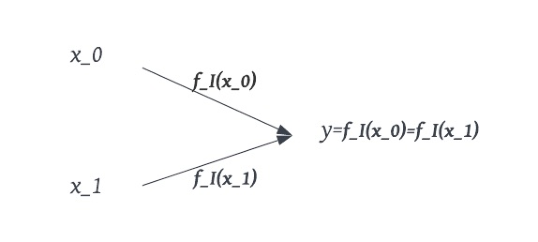
\includegraphics[]{figures/TCF.pdf}
	\caption{``A claw'' of a TCF function $f_{\mathcal{I}}(x)$ is a pair of $(x_0,x_1)$ such that $y=f_{\mathcal{I}}(x_0)=f_{\mathcal{I}}(x_1)$}\label{fig:TCF}
\end{figure}


Trapdoor claw-free functions (TCF), Fig.~\ref{fig:TCF}, is a 2-to-1 one-way function $f_\mathcal{I}(x)$ such that it is hard for a (quantum) polynomial-time adversary to simultaneously find the preimage pair $(x_0,x_1)$ \textit{``a claw''}, given any image $y = f_{\mathcal{I}}(x_0)=f_{\mathcal{I}}(x_1)$ where $\mathcal{I}$ is some problem instance. Sometimes, TCFs can also be defined as a pair of functions $f_{\mathcal{I},0}(x)$, $f_{\mathcal{I},1}(x)$ that are both injective and have the same image space and it is cryptographically hard to find two inputs mapping to the same output. One special property of TCFs is that given a problem instance $\mathcal{I}$ sampled together with a suitable trapdoor $t_{k}$, it is possible for one to find all the pre-images of $y$. More formally, we can define the trapdoor claw-free function as follows:
\begin{defn}[Trapdoor Claw-Free Function (TCF)]
    Let $\mathcal{X}$, $\mathcal{Y}$ be finite sets, we require the family of functions $\mathcal{F}$ satisfies the following properties:
\begin{itemize}
    \item For each public key $k$, there are two functions $\{f_{\mathcal{I},b}:\mathcal{X}\to\mathcal{Y}\}_{b\in\{0,1\}}$ that are both injective and have the same range, and are invertible given a suitable trapdoor $t_k$ (i.e.  $t_k$ can be used to efficiently compute $x$ given $b$ and $y=f_{\mathcal{I},b}(x)$). 
    \item The pair of functions should be \textit{claw-free}: it is hard to find the pair $(x_0,x_1)\in\mathcal{X}^2$ such that $y=f_{k,0}(x_0)=f_{k,1}(x_1)$.
\end{itemize}
\end{defn}

\noindent Note that a quantum device can not invert the function a find the claw $(x_0,x_1)$, it can hold these two preimages together with $y$ in a superposition
\begin{align}
    \frac{1}{\sqrt{2}}(\ket{x_0}+\ket{x_1})\ket{y}.
    \label{eq:tcfstate}
\end{align}
This is obtained by first preparing a uniform superposition over all $x\in\mathcal{X}$ via Hadamard transform
\begin{align}
    \frac{1}{\sqrt{\mathcal{X}}}\sum_{x\in\mathcal{X}}\ket{x},
\end{align}
then evaluating $f_{\mathcal{I},b}(x)$ into an output register to yield 
\begin{align}
    \frac{1}{\sqrt{\mathcal{X}}}\sum_{x\in\mathcal{X}}\ket{x}\ket{f_{\mathcal{I},b}(x)}.
\end{align}
If one measures the output register and obtains the result $y$, the state would collapse to the~\eqref{eq:tcfstate} state such that $y=f_{k,0}(x_0)=f_{k,1}(x_1)$.
Measuring the~\eqref{eq:tcfstate} state in the standard basis ($Z$ basis), one would obtain a random preimage as the measurement result, i.e. $m=x_0$ or $m = x_1$, but not both, since measuring a quantum state means collapsing that state to one possible outcome. Besides, measuring ~\eqref{eq:tcfstate} state in the $X$ basis yields a measurement result $m$ and a bit $c$ that satisfy $m \cdot (x_0\oplus x_1) = c$. This special property of TCFs could be used to construct a Proof of Quantumness protocol, the details of which will be discussed in section~\ref{proof_of_quantumness}.



However, a fully constructive Trapdoor Claw-Free (TCF) function that satisfies our cryptographic requirements has not been explored yet. The paper \cite{Brakerski18_Interactiveproofofquantumness} considers a ``relaxed'' version of the TCFs, referred to as \textbf{Noisy trapdoor claw-free functions (NTCFs)}. In NTCFs, the range of functions $f_{k,0}$ and $f_{k,1}$ is represented by a distribution $\mathcal{D}$ over $\mathcal{Y}$, denoted as $\mathcal{D}_{\mathcal{Y}}$. In other words, each function returns a density rather than a point. Instead of considering the range of $f{k,b}$, we consider the support of the output densities, $\mathsf{SUPP}(f_{\mathcal{I},b}(x))$. If $y$ lies in this support, a party that holds the trapdoor $t_k$ can use it to invert the function and find the preimages of $y$.

\begin{defn}[Noisy Trapdoor Claw-Free family]
   Let $\lambda$ be a security parameter. Let $\mathcal{X}$ and $\mathcal{Y}$ be finite sets. Let $\mathcal{K}_{\mathcal{F}}$ be a finite set of keys. A family of functions
   \begin{align}
       \mathcal{F}=\{f_{\mathcal{I},b}:\mathcal{X}\to \mathcal{D}_{\mathcal{Y}}\}_{b\in\{0,1\}}
   \end{align}
is called a noisy trapdoor claw-free (NTCF) family if the following conditions hold:
\begin{enumerate}
    \item \textbf{Efficient Function Generation.} There exists an efficient probabilistic algorithm $\mathsf{GEN}_{\mathcal{F}}$ which generates problem instance $\mathcal{I}$ together with a trapdoor $t_{k}$:
    \begin{align}
        \mathsf{GEN}_{\mathcal{F}}(1^{\lambda})\to (\mathcal{I},t_k).
    \end{align}
    \item \textbf{Trapdoor Injective Pair.}
    \begin{itemize}
        \item \textit{Trapdoor:} There exists an efficient deterministic algorithm \textit{Invert} $\mathsf{INV}_\mathcal{F}$ such that with overwhelming probability over the choice of $(\mathcal{I},t_k)$, the following holds:
        \begin{center}
            for all $b\in\{0,1\}$, $\mathbf{x}\in \mathcal{X}$ and $y\in \mathsf{SUPP}(f_{\mathcal{I},b}(x))$, $\mathsf{INV}_\mathcal{F}(t_k,b,y)=x$.
        \end{center}
        \item \textit{Injective pair:} There exists a perfect matching set for an instance $\mathcal{I}$ denoted  $\mathcal{R}_{\mathcal{I}}\subseteq \mathcal{X}\times \mathcal{X}$ such that $f_{\mathcal{I},0}(x_0)=f_{\mathcal{I},0}(x_1)$ if and only if $(x_0,x_1)\in \mathcal{R}_{\mathcal{I}}$. 
    \end{itemize}
    \item \textbf{Efficient Range Superposition.} For all keys $k\in \mathcal{K}_{\mathcal{F}}$ and $b\in\{0,1\}$ there exists a function $f'_{\mathcal{I},b}:\mathcal{X}\to \mathcal{D}_{\mathcal{Y}}$ such that the following hold:
    \begin{itemize}
        \item For all $(x_0,x_1)\in \mathcal{R}_k$ and $y\in\mathsf{SUPP}(f'_{\mathcal{I},b})(x_b)$, $\mathsf{INV}_{\mathcal{F}}(t_k,b\oplus 1,y)=x_{x\oplus 1}$.
        \item There exists an efficient deterministic procedure $\mathsf{CHK}_{\mathcal{F}}$ that given set of input $\mathcal{I}$, $b\in\{0,1\}$, $x\in \mathcal{X}$ and $y\in \mathcal{Y}$, check whether $y$ is an element of the support of $f$ or not. This procedure returns $1$ if $y\in \mathsf{SUPP}(f'_{\mathcal{I},b}(x))$ and $0$ otherwise. 
        %Note that $\mathsf{CHK}_{\mathcal{F}}$ is not provided the trapdoor $t_{k}$.
        \item 
        %For every $k$ and $b\in\{0,1\}$,
        %$$E_{x\gets_U \mathcal{X}}[H^2(f_{\mathcal{I},b}(x),f'_{k,b}(x))]\leq 1/50.$$
        %Here $H^2$ is the Hellinger distance. Moreover, 
        There exists an efficient procedure $\mathsf{SAMP}_{\mathcal{F}}$ that on input the problem instance $\mathcal{I}$ and $b\in\{0,1\}$, prepares the state
        \begin{align}
            \displaystyle{\frac{1}{\sqrt{|\mathcal{X}|}}}\sum_{x\in\mathcal{X},y\in\mathcal{Y}}\sqrt{(f'_{\mathcal{I},b}(x)(y))}|x\rangle|y\rangle.
        \end{align}
    \end{itemize}
    \item \textbf{Claw-free Property.} There no probabilistic polynomial time adversary $\mathcal{A}$ can find the ``claw'' $(x_0,x_1,y)$. More formally, there exists a negligible function $\mathsf{negl}(\cdot)$ such that the following holds:
    \begin{align}
        \Pr[(x_0,x_1)\in\mathcal{R}_{\mathcal{I}}:(\mathcal{I},t_k)\gets \mathsf{GEN}_{\mathsf{F}}(1^{\lambda}),(x_0,x_1)\gets \mathcal{A}(\mathcal{I)}]\leq \mathsf{negl}(\lambda).
    \end{align}
\end{enumerate}
\end{defn}

\subsubsection{TCFs from LWE}
For a matrix $\mathbf{A}\in\mathbb{Z}^{m\times n}_q$ and vectors $\mathbf{s},\mathbf{e}\in\{0,1\}^n$, consider the LWE instance $(\mathbf{A},\mathbf{A}\mathbf{s}+\mathbf{e})$ with the trapdoor $t_k=\{\mathbf{s},\mathbf{e}\}$. We can define the TCFs family by letting $f_{\mathcal{I},0}(\mathbf{x})=\mathbf{A}\mathbf{x}+\mathbf{e}_0$ and $f_{\mathcal{I},1}(\mathbf{x})=\mathbf{A}(\mathbf{x}+\mathbf{s})+\mathbf{e}_0+\mathbf{e}$. If $\mathbf{e}_0 =\bf{0}$, then $f_{\mathcal{I},1}(\mathbf{x})=f_{\mathcal{I},0}(\mathbf{x}+\mathbf{s})$; however, we need to hide the information of $\mathbf{x}$, it is essential to sample $\mathbf{e}_0$ from a Gaussian distribution much wider than $\mathbf{e}$ such that it ensures that the distribution of $f_{\mathcal{I},1}(\mathbf{x})$ and $f_{\mathcal{I},0}(\mathbf{x}+\mathbf{s})$ are statistically close as per the requirements of the NTCFs defined in the previous subsection.

Based on this idea,~\cite{Brakerski18_Interactiveproofofquantumness} built a NTCFs family from the LWE problem as follows:

\begin{defn}[TCFs based on LWE~\cite{Brakerski18_Interactiveproofofquantumness}\label{defn:tcfsfromlwe}]
    Let $\lambda$ be a security parameter. Let $q\geq 2$ be a prime and $\ell,n,m\geq 1$ are polynomially bounded functions of $\lambda$, and $B_L,B_V, B_P$ be positive integers such that the following conditions hold:
    \begin{itemize}
        \item $n=\Omega(\ell\log q +\lambda)$,
        \item $m=\Omega(n\log q)$,
        \item $B_P = \displaystyle{\frac{q}{2C_T\sqrt{mn\log q}}}$, for $C_T$ is a universal constant in the $\mathsf{GenTrap}$ algorithm.
    %\item We have $B_L<B_V<B_P$ so that the ratios $\frac{B_P}{B_V}$ and $\frac{B_V}{B_L}$ are both super-polynomial in $\lambda$.
    \end{itemize}
\begin{enumerate}
    \item \textbf{Efficient Function Generation:} The $\mathsf{GEN}_{\mathcal{F}}(1^{\lambda})$ is constructed as follows:
    \begin{itemize}
        \item Using the trapdoor mechanism  $\mathsf{GenTrap}(1^n,1^m,q)$ to return a matrix $\mathbf{A}\in\mathbb{Z}^{m\times n}_q$ and a trapdoor $t_{k}=\mathbf{R}$, $m\geq \Omega (n\log q)$ such that the distribution of $\mathbf{A}$ is negligibly (in $n$) close to the uniform distribution on $\mathbb{Z}^{m\times n}_q$.
        \item Sample a uniformly random $\mathbf{s}\gets \{0,1\}^{n}$ and a vector $\mathbf{e}\gets \mathbb{Z}^m_q$ from the distribution $D^m_{\mathbb{Z}_q,B_V}$.
        \item $\mathsf{GEN}_{\mathcal{F}}(1^{\lambda})$ returns 
        \begin{align}
            (\mathcal{I},t_{k})=((\mathbf{A},\mathbf{A}\mathbf{s}+\mathbf{e}),t_{k}=\mathbf{R}.
        \end{align}
    Note that the trapdoor $t_{k}=\mathbf{R}$ can be referred to as a ``strong'' trapdoor since it can be used to reconstruct $\mathbf{s}$ and $\mathbf{e}$. In most existing cryptographic constructions using NTCFs, for simplicity, the trapdoor is usually set as $t_{k}=(\mathbf{s},\mathbf{e})$.
    \end{itemize}
    \item \textbf{Trapdoor Injective Pair}
    \begin{itemize}
        \item For any pair $(\mathcal{I},t_{k})=((\mathbf{A},\mathbf{A}\mathbf{s}+\mathbf{e}),t_{k}=(\mathbf{s},\mathbf{e})$, a bit $b\in\{0,1\}$, the density function of $f_{\mathcal{I},b}(\mathbf{x})$ is defined as follows:
        \begin{align}
            \forall \mathbf{y}\in\mathcal{D}_{\mathcal{Y}},(f_{\mathcal{I},b}(\mathbf{x}))(\mathbf{y})=\mathcal{D}^{m}_{\mathbb{Z}_q,B_P}(\mathbf{y}-\mathbf{A}(\mathbf{x}+b\mathbf{s}))
        \end{align}
        where $\mathbf{y}\in\mathbb{Z}^m_q$. The support of the density function $f_{\mathcal{I},b}(\mathbf{x})$ is 
        \begin{align}
            \mathsf{SUPP}(f_{\mathcal{I},0}(\mathbf{x}))=\{\mathbf{A}\mathbf{x}+\mathbf{e}_0:\|\mathbf{e}_0\|\leq B_P\sqrt{m}\}.
        \end{align}
        \begin{align}
             \mathsf{SUPP}(f_{\mathcal{I},0}(\mathbf{x}))=\{\mathbf{A}(\mathbf{x}+\mathbf{s})+\mathbf{e}_0:\|\mathbf{e}_0\|\leq B_P\sqrt{m}\}.
        \end{align}
        
    The inversion algorithm $\mathsf{INV}_\mathcal{F} \equiv \mathsf{INVERT}(t_{k}, \mathbf{A}, \mathbf{y})$ finds $(\mathbf{s}_0, \mathbf{e}_0)$ such that $\mathbf{y} = \mathbf{A}\mathbf{s}_0 + \mathbf{e}_0$ and returns $\mathbf{s}_0 - b \cdot \mathbf{s} \in \mathcal{X}$. Due to the parameter selections and the choice of $\mathbf{e}_0$, we have that $\mathsf{INV}_\mathcal{F}$ returns a preimage of the NTCFs.
       
       We have that, for all $\mathbf{y}\in \mathsf{SUPP}(f_{\mathcal{I},b}(\mathbf{x}))$, $\mathsf{INVERT}(t_{k},\mathbf{A},\mathbf{y})=\mathbf{x}+b\mathbf{s}$. Hence, it follows that $\mathsf{INV}_\mathcal{F}(t_{k},b,\mathbf{y})=\mathbf{x}$.
        
        \item \textit{Injective pair:} Let $\mathcal{I}=(\mathbf{A},\mathbf{A}\mathbf{s}+\mathbf{e})$. From the construction, it follows that $f_{\mathcal{I},0}(\mathbf{x}_0)= f_{\mathcal{I},0}(\mathbf{x}_1)$ if and only if $\mathbf{x}_1=\mathbf{x}_0+\mathbf{s}$. Also, the matching set is defined as $\mathcal{R}_{\mathcal{I}}=\{(\mathbf{x},\mathbf{x}+\mathbf{s})|\mathbf{x}\in \mathbb{Z}^n_q\}$.
    \end{itemize}
    \item \textbf{Efficient Range Superposition} 
    
    On input $(\mathbf{A},\mathbf{A}\mathbf{s}
    +\mathbf{e})$, $b\in\{0,1\}$, $\mathbf{x}\in \mathbb{Z}^n_q$ and $\mathbf{y}\in \mathbb{Z}^m_q$, the procedure $\mathsf{CHK}_{\mathcal{F}}$ operates as follows.
    \begin{itemize}
        \item If $b=0$, it computes $\mathbf{e}'=\mathbf{y}-\mathbf{A} \mathbf{x}$. If $\|\mathbf{e}'\|\leq B_P\sqrt{m}$, the procedure outputs $1$, else output $0$.
        \item If $b=1$, it computes $\mathbf{e}'=\mathbf{y}-\mathbf{A}\mathbf{x} -(\mathbf{A}\mathbf{s}+\mathbf{e})$. If $\|\mathbf{e}'\|\leq B_P\sqrt{m}$, the procedure outputs $1$, else output $0$.
    \end{itemize}

    The procedure $\mathbf{SAMP}_{\mathcal{F}}$ prepares the quantum state as per the following steps:
    \begin{itemize}
        \item Create the following superposition:
        \begin{align}
            \sum_{\mathbf{e}_0\in\mathbf{Z}^m_q} \sqrt{\mathcal{D}_{\mathbb{Z}^m_q,B_P}(\mathbf{e}_0)}\ket{\mathbf{e}_0}.
        \end{align}
        \item Create a uniform superposition over $\mathbf{x}\in\mathbf{Z}^n_q$ to obtain the state:
        \begin{align}
            \frac{1}{\sqrt{q^m}}\sum_{\mathbf{x}\in\mathbb{Z}^n_q,\mathbf{e}_0\in\mathbf{Z}^m_q} \sqrt{\mathcal{D}_{\mathbb{Z}^m_q,B_P}(\mathbf{e}_0)}\ket{\mathbf{x}}\ket{\mathbf{e}_0}.
        \end{align}
        \item Now, using the problem instance $\mathcal{I}=(\mathbf{A},\mathbf{A}\mathbf{s}+\mathbf{e})$ and the bit $b$ to create the state
        \begin{align}
            \frac{1}{\sqrt{q^m}}\sum_{\mathbf{x}\in\mathbb{Z}^n_q,\mathbf{e}_0\in\mathbf{Z}^m_q} \sqrt{\mathcal{D}_{\mathbb{Z}^m_q,B_P}(\mathbf{e}_0)}\ket{\mathbf{x}}\ket{\mathbf{e}_0}\ket{\mathbf{A}\mathbf{x}+\mathbf{e}_0+b\cdot (\mathbf{A}\mathbf{s}+\mathbf{e})}  
        \end{align}
        \item Since $\mathbf{e}_0$ can be computed from $x$ and the last register, $b$ and the problem instance $\mathcal{I}$, one can uncompute the register containing $\mathbf{e}_0$ and obtain the state
        \begin{align}
            &\frac{1}{\sqrt{q^m}}\sum_{\mathbf{x}\in\mathbb{Z}^n_q,\mathbf{e}_0\in\mathbf{Z}^m_q} \sqrt{\mathcal{D}_{\mathbb{Z}^m_q,B_P}(\mathbf{e}_0)}\ket{\mathbf{x}}\ket{\mathbf{A}\mathbf{x}+\mathbf{e}_0+b\cdot (\mathbf{A}\mathbf{s}+\mathbf{e})}\\
            &=\frac{1}{\sqrt{q^m}}\sum_{\mathbf{x}\in\mathbb{Z}^n_q,\mathbf{e}_0\in\mathbf{Z}^m_q} \sqrt{(f_{\mathcal{I},b}')(\mathbf{y})}\ket{\mathbf{x}}\ket{\mathbf{y}}.
            \label{eq:LWEtcfqstate}
        \end{align}
        
    \end{itemize}
     
    \item \textbf{Claw-free Property} Suppose there exists an adversary $\mathcal{A}$, on input $\mathbf{y}=\mathbf{A}\mathbf{s}+\mathbf{e}$ can output the pair $(\mathbf{x}_0,\mathbf{x}_1)\in\mathcal{R}_k$. This adversary can be used to break the $\mathsf{LWE}$ problem since $\mathbf{x}_1-\mathbf{x}_0=\mathbf{s}$.
    
\end{enumerate}
\end{defn}


\subsubsection{TCFs from RLWE}
Two years later from the first definition of the NTCFs from LWE was published, Brakerski continued his work in~\cite{BrakerskiProofofQuantumness} and showed that using the ring version of the LWE problem yeild better results since RLWE-based primitives exhibit greater efficiency and yield smaller key sizes than their LWE-based counterparts, due to the ring dimension. 
%This dimension plays a crucial role in determining the size of the challenge space. The larger the challenge space, the less the soundness error of the scheme has and the fewer times the underlying protocol has to repeat. 

\begin{defn}[TCFs from RLWE problem~\cite{BrakerskiProofofQuantumness}] Let $\lambda$ be the security parameter, $n=2^{\log \lambda}$. Set
\begin{itemize}
    \item Ring $R=\mathbb{Z}[x]/(x^n+1)$.
    \item Modulus $q=\mathsf{poly}(n)$, $R_q=R/qR$.
    \item $m=\Omega(\log q)$: determines the dimension of range space
    $\chi = D_{\mathbb{Z}^n_q,B_V}$: the noise distribution.
    \item $B_P$: the noise bound for function evaluation satisfies the constraints:
    \begin{itemize}
        \item $B_P\geq \Omega(nmB_V)$,
        \item $2B_P\sqrt{nm}\leq q/(C_T\sqrt{n\log q})$ for some constant $C_T$.
    \end{itemize}
    The domain is $R_q=\mathbb{Z}_q[x]/(x^n+1)$ and the range is $R_q^{m}$.\\
    The problem instance $\mathcal{I}=(\mathbf{a},\mathbf{a}\cdot s+\mathbf{e})$, where $s\in R_q$, $a_i,e_i\in R_q$ for all $i\in[m]$, $\mathbf{a}=[a_1,\dots,a_m]^T$, $\mathbf{e}=[e_1,\dots,e_m]^T$.\\
    For $b\in\{0,1\}$, the density function $f_{\mathcal{I},b}(x)$ is defined as follows:
    \begin{align}
        \forall \mathbf{y}\in R_q^m, (f_{\mathcal{I},b}(x))(\mathbf{y})=D_{\mathbb{Z}^{nm},B_P}(\mathbf{y}-\mathbf{a}\cdot x - b\cdot \mathbf{a}\cdot s),
    \end{align}
    where $\mathbf{y}=[y_1,\dots,y_m]^T$, and each $y_i$ can be represented as element in $\mathbb{Z}^n_q$; similarly for $\mathbf{a}\cdot x$ and $\mathbf{a}\cdot s$.
\end{itemize}
\begin{enumerate}
    \item \textbf{Efficient Key Generation} 
        \begin{itemize}
            \item The algorithm $\mathsf{GenTrap}(1^n,1^m,q)$ returns $\mathbf{a}\in R^m_q$ and a trapdoor $t_{k}$ such that the distribution of $\mathbf{a}$ is negligibly (in $n$) close to the uniform distribution on $R^m_q$.
        \item Sample a uniformly random $\mathbf{s}\gets R^q$ and a vector $\mathbf{s}\gets \chi$.
        \item Compute $\mathbf{a}\cdot s+\mathbf{s}$.
        \item $\mathsf{GEN}_{\mathcal{F}}(1^{\lambda})$ returns \begin{align}
            (\mathcal{I},t_k)=((\mathbf{a},\mathbf{a}\cdot s+\mathbf{s}),(t_{k},s)).
        \end{align}
        \end{itemize}
    \item \textbf{Trapdoor Injective Pair}
        \begin{itemize}
        \item The support of the density function of $f_{\mathcal{I},b}(x)$ is 
        \begin{align}
            \mathsf{SUPP}(f_{\mathcal{I},b}(x))=\{\mathbf{y}\in R_q^m:\|\mathbf{y}- \mathbf{a} \cdot x-b\cdot \mathbf{a} \cdot s\|\leq B_P\sqrt{nm}\}.
        \end{align}
        For $\mathcal{I}=(\mathbf{a},\mathbf{a}\cdot s+\mathbf{e})$, the inversion algorithm $\mathsf{INV}_\mathcal{F}(t_{k},b,\mathbf{y}\in R_q^m) \equiv \mathsf{INVERT}(t_{k},\mathbf{a},\mathbf{y})-b\cdot s$. We have that, for all $\mathbf{y}\in \mathsf{SUPP}(f_{\mathcal{I},b}(x))$, $\mathsf{INVERT}(t_{k},\mathbf{a}\,y)=x+b\cdot s$. Hence, it follows that $\mathsf{INV}_\mathcal{F}(t_{k},b,\mathbf{y})= x$.
        
        \item \textit{Injective pair:} From the construction, it follows that $f_{\mathcal{I},0}(x_0)= f_{\mathcal{I},0}(x_1)$ if and only if $x_1=x_0+s$. Denote the matching set $\mathcal{R}_{\mathcal{I}}=\{(x,x+s)|x\in R_q\}$.
    \end{itemize}
    \item \textbf{Efficient Range Superposition}
    Perform similar operations as NTCFs from LWE, on input $(\mathbf{a},\mathbf{a}\cdot s+\mathbf{s})$, $b\in\{0,1\}$, $x\in R^q$ and $\mathbf{y}'\in R^m_q$, the procedure $\mathsf{CHK}_{\mathcal{F}_{\mathsf{RLWE}}}$ outputs $1$ if $\mathbf{y}\in\mathsf{SUPP}(f'_{\mathcal{I},b}(x))$ and $0$ otherwise.
    Note that the condition that $\mathsf{CHK}_{\mathcal{F}_{\mathsf{RLWE}}}$ needs to check is $\|\mathbf{y}'-\mathbf{a}\cdot x - b\cdot \mathbf{y}\|\leq B+P\sqrt{n\cdot m}$.
    The procedure $\mathbf{SAMP}_{\mathcal{F}}$ prepares the quantum states similar to the one built on LWE in the previous section.
     
    \item \textbf{Claw-free Property} Suppose there exists an adversary $\mathcal{A}$, on input $\mathbf{y}=\mathbf{a}\cdot s+\mathbf{s}$ can output the pair $(x_0,x_1)\in\mathcal{R}_k$. This adversary can be used to break the $\mathsf{RLWE}$ problem since $x_1-x_0=s$.  
        
    \end{enumerate}
\end{defn}

\subsection{Adaptive hardcore bit property for TCFs from LWE}

Recall that in the TCFs from LWE, measuring the output register of the~\eqref{eq:LWEtcfqstate} state, obtaining the measurement outcome $\mathbf{y}$ and the superposition
\begin{align}
    \frac{1}{\sqrt{2}}(|\mathbf{x}_0\rangle +|\mathbf{x}_1\rangle)|\mathbf{y}\rangle.\label{eq:lwetfcstate}
\end{align}
\noindent Recall that when measuring the $\mathbf{x}$ register in the X basis, we obtain the measurement result $m\in\{0,1\}^n$ and a bit $c\in\{0,1\}$ such that $m\cdot(\mathbf{x}_0+\mathbf{x}_1) = c$. This equation provides some information about both preimages. Note that~\cite{Brakerski18_Interactiveproofofquantumness} used the LWE-based hardness assumption, where $\mathbf{x}_0 + \mathbf{x}_1 = \mathbf{s}$, where $\mathbf{s}$ is some fixed secret determined by the problem instance $\mathcal{I}$. Hence, measuring the first register in the Hadamard basis yields a uniformly random $m$ such that $m\cdot \mathbf{s} = c$. If we repeat the entire procedure $O(n)$ times yield linearly independent such $m$, which suffices to recover $\mathbf{s}$ with high probability. Hence, we need the structure of the function $f$ to be a little more complicated so that even with $\mathbf{x}_0, \mathbf{x}_1 =\mathbf{x}_0- \mathbf{s}$, and given many ``equations'' $m$ could be useless since without additional knowledge of a preimage, one cannot determine what the equation is about. This is why we need the trapdoor claw-free function to satisfy the \textbf{hardcore bit}, which is similar to a one-way function. Specifically, $m\cdot(\mathbf{x}_0+\mathbf{x}_1) = c$ is the hardcore bit that ensures it is ``hard'' to compute a bit of $\mathbf{x}_0$ or $\mathbf{x}_1$ given $\mathbf{y}$. Moreover, if the adversary can simultaneously find this predicate and a preimage $\mathbf{x}_b$, it could find the whole claw $(\mathbf{x}_0, \mathbf{x}_1)$.



\noindent\textbf{Why does IPOF~\cite{Brakerski18_Interactiveproofofquantumness} construction use the term ``adaptive'' for the hardcore bits property?}
Combining all the mentioned requirements, we can write the hardcore bit property for the LWE-based trapdoor claw-free function as follows:
Given a trapdoor claw-free function $f_{\mathcal{I},b}(\mathbf{x})$, a hardcore bit for $f$ is a $1$-output-bit function $h$ such that given  $f_{\mathcal{I},b}(\mathbf{x})$ (but not $\mathbf{x}$) it is hard to predict $h$. Here, the hardcore bit that underlies the assumption is the function $c = h(x)= m\cdot (\mathbf{x}_0 + \mathbf{x}_1)$ for any $m$.
Since this equation can be rewritten as $m'\cdot \mathbf{s} =c$. The property can be stated as it is hard to produce the string $m'$ that satisfies the above equation.

Moreover, we allow the adversary $\mathcal{A}$ to \textbf{\textit{adaptively choose the string $m'$}}. This also means that more power is given to the adversary. It is in this sense that the hardcore bit property is \textbf{adaptive}. Concretely, in the LWE-based construction, even the adversary $\mathcal{A}$ can adaptively choose the string $m$ after being given access to the LWE sample $\mathbf{A}\mathbf{s}+\mathbf{e}$, i.e. the choice of $m'$ depend upon the LWE sample, due to the \textit{leakage resilience} property of the LWE problem, the information of the $\mathbf{s}$ remains secret. The idea is that instead of sampling a uniformly random matrix $\mathbf{A}\in\mathbb{Z}^{m\times n}_q$ together with its trapdoor, we replace $\mathbf{A}$ by a ``lossy mode'' $\tilde{\mathbf{A}}$, where $\tilde{\mathbf{A}}$ is sampled from a special distribution so that $\tilde{\mathbf{A}}=\mathbf{B}\mathbf{C}+\mathbf{E}$ for a skinny matrix $\mathbf{B}$, a wide matrix $\mathbf{C}$ and $\mathbf{E}\gets\chi^{m\times n}$. It holds that $\tilde{\mathbf{A}}$ is indistinguishable from $\mathbf{A}$. Now, when we multiply $\tilde{\mathbf{A}}$ by $\mathbf{s}$, the matrix $\mathbf{C}$ compresses the information of $\mathbf{s}$. To be more specific, provided the matrix $\mathbf{C}$ is a uniformly random matrix with sufficiently few rows, the distribution $(\mathbf{C},\mathbf{C}\mathbf{s})$ for an arbitrary secret $\mathbf{s}$ does not reveal any parity of $\mathbf{s}$. More information on the proof can be found in~\cite{Brakerski18_Interactiveproofofquantumness}.
\section{Proof of Quantumness} \label{proof_of_quantumness}

\subsection{Interactive proof}
A proof serves as a means of persuading someone that a specific statement is true. We typically involve two parties when discussing proofs: \textit{a prover} and \textit{a verifier}. The prover aims to convince the verifier of the validity of a given statement, while the verifier's goal is to accept only accurate assertions. Before giving the definition of the interactive proof, we first recall that a language is simply a set of strings $L\subseteq \{0,1\}^*$. The definition of an interactive proof for a statement $x$ in a language $L$ is defined as follows:

\begin{defn}[Interactive proof]
    An interactive proof system for a language $L$ is a protocol between a computationally unrestricted prover $\mathcal{P}$ and a polynomial-time verifier $\mathcal{V}$ such that on input a statement $x$:
    \begin{itemize}
        \item \textbf{Completeness}: If $x\in L$, then an honest prover $\mathcal{P}$ that follows protocol should be able to convince the verifier $\mathcal{V}$ about the validity of the statement. 
        $$\forall x\in L, \Pr[(\mathcal{V}\leftrightarrow \mathcal{P})(x) \text{accepts }]=1.$$
        \item \textbf{Soundness $\epsilon$:} If $x \notin L$, then no malicious prover $\mathcal{P}'$ should be able to convince $\mathcal{V}$  with a success probability greater than $\epsilon$.
        $$\forall x\notin L, \forall \mathcal{P}', \Pr[(\mathcal{V}\leftrightarrow \mathcal{P}')(x) \text{accepts}]\leq \epsilon.$$
    \end{itemize}
\end{defn}
\begin{figure}[!htb]
	\centering
	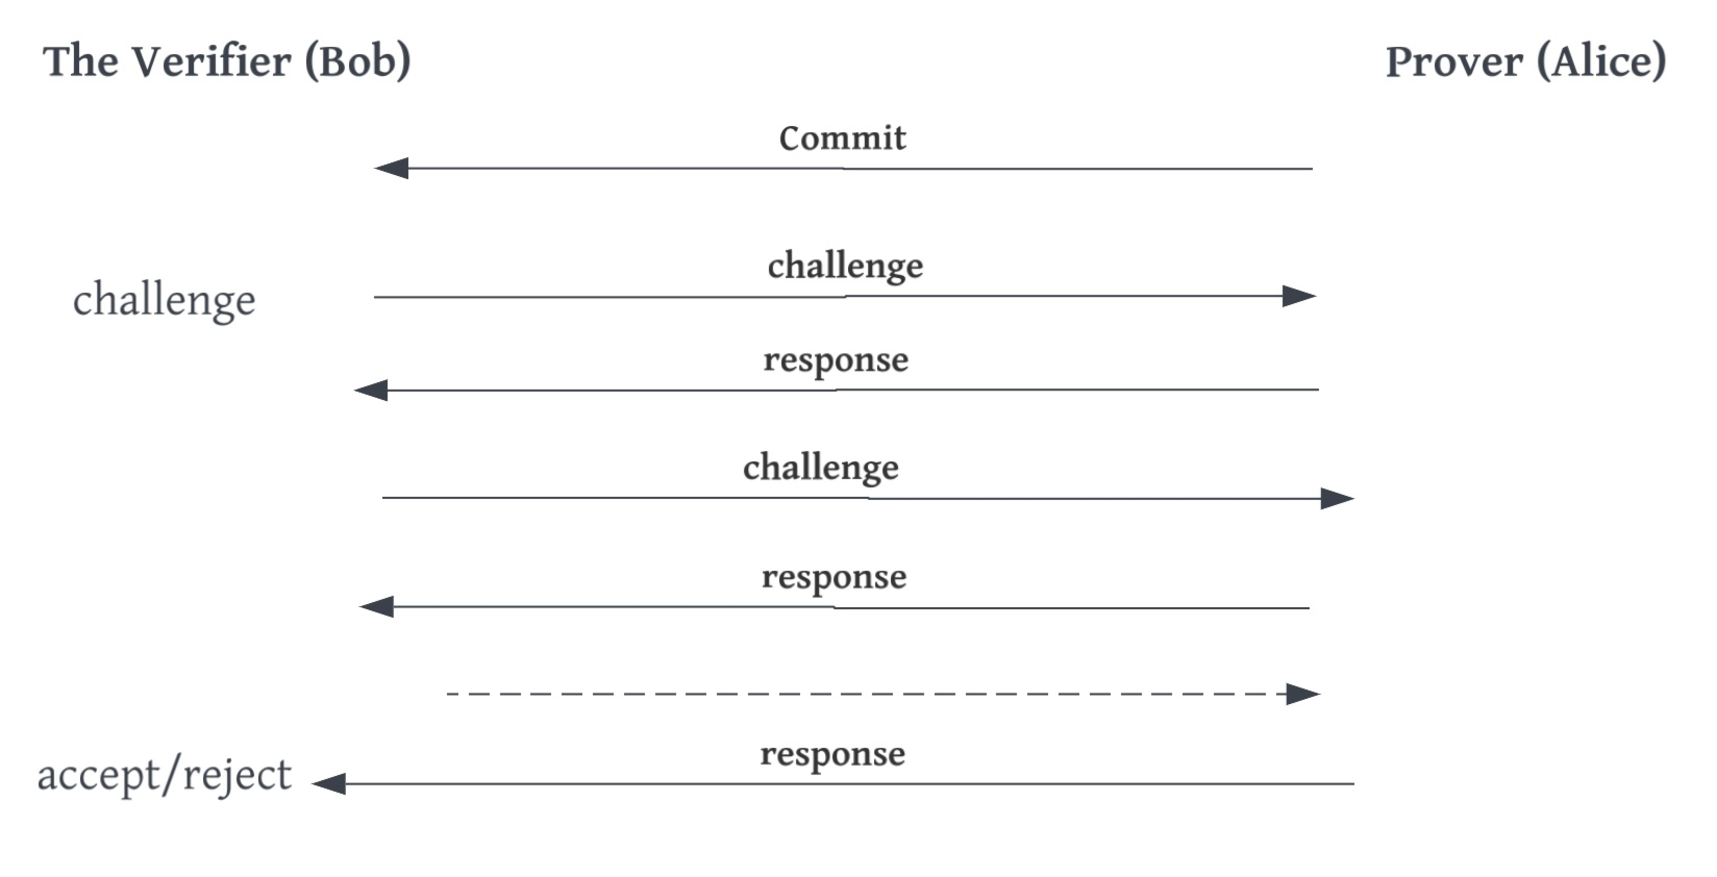
\includegraphics[scale = 0.35]{figures/IP.pdf}
	\caption{An interactive proof between a prover (Alice) and a verifier (Bob) typically has three main phases: commit, challenge, and response. The protocol may repeat the challenge-response phase multiple times to ensure the soundness property.}\label{fig:ip}
\end{figure}

\subsection{Proof of quantumness}
In recent years, under the efforts of building quantum computers, the verification of quantum behaviour has become significantly crucial. This underscores the necessity for a protocol in which a classical party can efficiently certify the quantum advantage of an untrusted device - the Proof of Quantumness. An interactive proof of quantumness~\cite{Brakerski18_Interactiveproofofquantumness,experiment_interactive_PoQ} is an interactive quantum verification protocol between two parties: a quantum prover $\mathcal{P}$ and a classical verifier $\mathcal{V}$. The verifier $\mathcal{V}$'s goal is to test the ``quantumness'' of the prover through an exchange of classical information. A common recent approach is to build the Interactive Proof of Quantumness protocol using TCFs.

%\begin{defn}[Proof of Quantumness~\cite{liu22poqdefn}]
%     A proof of quantumness is an interactive protocol with an efficient classical verifier satisfying:
%     \begin{itemize}
%         \item \textbf{Completeness.} There exists a polynomial-time quantum prover that can convince the verifier about its ``quantum'' ability.
%         \item \textbf{Soundness} $\epsilon$.
%          Any polynomial-time classical prover convinces the verifier with probability at most $\epsilon + \mathsf{negl}$ for some negligible function $\mathsf{negl}$.
%     \end{itemize}
%\end{defn}

\subsection{LWE}
The basic idea of employing the TFCs from LWE (Definition~\ref{defn:tcfsfromlwe}) to build the interactive proof of quantumness protocol is presented as follows:
\begin{enumerate}
    \item The verifier samples an LWE instance $\mathcal{I}=(\mathbf{A},\mathbf{y}=\mathbf{A}\mathbf{s}+\mathbf{e})$ together with a trapdoor $t_{k}=(\mathbf{s},\mathbf{e})$, and sends $\mathcal{I}$ and the description of the NTCFs $f_{\mathcal{I}}(\cdot)$ to the prover.
    \item The prover then:
    \begin{itemize}
        \item prepares a uniform superposition over $\mathbf{x}\in\{0,1\}^n$
        \begin{align}
            \frac{1}{\sqrt{2}^n}\sum_{\mathbf{x}\in\{0,1\}^n}\ket{\mathbf{x}},
        \end{align}
        \item evaluates $f_\mathcal{I}(\cdot)$ into an output register yields the state
        \begin{align}
            \sum_{\mathbf{x}\in\{0,1\}^n}\ket{\mathbf{x}}\ket{f_{\mathcal{I}}(\mathbf{x})},
        \end{align}        
        \item measures the output register to obtain $\mathbf{w}\in\mathcal{Y}$.
    The prover sends $\mathbf{w}$ to the verifier as the commitment for its quantum power.
    \end{itemize}
    \item The remaining state after measuring on the output register of the prover now is
    \begin{align}
        \frac{1}{\sqrt{2}}(\ket{\mathbf{x}_0}+\ket{\mathbf{x}_1})
    \end{align}
    where $\mathbf{x}_0$, $\mathbf{x}_1$ are two preimages of $\mathbf{w}$.
    \item The verifier challenge by asking the prover to measure on either the standard basis ($Z$ basis) $b=0$ or the Hadamard basis ($X$ basis) $b=1$.
    \item According to the verifier's challenge, the measurement outcome of the prover's state is:
    \begin{itemize}
        \item Standard basis: either $m=\mathbf{x}_0$ or $m=\mathbf{x}_1$, 
        \item Hadamard basis: $(c\in\{0,1\},m\in\{0,1\}^n)$ such that $m\cdot(\mathbf{x}_0+\mathbf{x}_1)=c$.
    \end{itemize}
    \item The verifier checks these tests: 
    \begin{itemize}
        \item Standard basis: simply check that $f_{\mathcal{I}}(m)=\mathbf{w}$.
        \item Hadamard basis: the verifier can recover $\mathbf{x}_0$, $\mathbf{x}_1$ from $\mathbf{y}$ using the trapdoor $t_k=(\mathbf{s},\mathbf{e})$, and check whether the pair $(m,c)$ satisfies $m\cdot(\mathbf{x}_0+\mathbf{x}_1)=c$.
    \end{itemize}

The protocol proceeds for $\lambda$ rounds. At the end of each round, the verifier samples a new problem instance and sends the new public key to the prover.
In a recent paper by Zhu~\cite{experiment_interactive_PoQ}, for each of the verifier’s possible choices, the experiment is repeated approximately $10^3$ times to collect statistics. 
\end{enumerate}

\begin{figure*}[!htp]
	\centering
	\begin{subfigure}[c]{\linewidth}
			\begin{quantikz}
\lstick{$f$} \setwiretype{c} & \gategroup[3,steps=7,style={rounded
    corners,fill=blue!10,draw=blue!50, inner
    xsep=5pt},background]{} & & & & \ctrl{0} & \setwiretype{n} & & & \lstick{$\mathsf{chall}$} & \setwiretype{c} \gategroup[3,steps=4,style={rounded
    corners,fill=blue!10,draw=blue!50, inner
    xsep=5pt},background]{} & & \ctrl{0} & \setwiretype{n} & \\
\setwiretype{n} & & \lstick{$\ket{\mathbf{0}}$} & \setwiretype{q} \qwbundle{n} & \gate{H^{\otimes n}} & \gate[2][5em]{U_f}\gateinput{$\mathbf{x}$}\gateoutput{$\mathbf{x}$}\wire[u]{c} & \qwbundle{n} & & & & & \qwbundle{n} & \gate{H^{\otimes n}}\wire[u]{c} & \meter{} & \setwiretype{c} \rstick{$\mathbf{m}$} & \setwiretype{n} & \\
\setwiretype{n} & & \lstick{$\ket{\mathbf{0}}$} & \setwiretype{q} \qwbundle{n-1} & & \gateinput{$\mathbf{y}$}\gateoutput{$\mathbf{y}\oplus f(x)$} & \qwbundle{n-1} & \meter{} & \setwiretype{c} \rstick{$\mathbf{w}$} & \setwiretype{n} & & & & & &
\end{quantikz}

			\caption{Two-round IPQ protocol, where $f$ is the TCF problem instance specified by the verifier. The prover executes the first round of the protocol, measuring the $\mathbf{y}$ register to obtain classical outcome $\mathbf{w}$. After receiving $\mathbf{w}$ from the prover the verifier communicates a random measurement basis $Z$ or $X$ for the prover to measure the $\mathbf{x}$ register in, yielding outcome $m\in\{0,1\}^n$. With knowledge of the problem instance's secret trapdoor, the verifier can efficiently verify the prover's response.}
	\end{subfigure}\label{fig:ipqlwe}
 \\
	\begin{subfigure}[c]{\linewidth}
		\begin{quantikz}
\lstick{$f$} \setwiretype{c} & \gategroup[3,steps=9,style={rounded
    corners,fill=blue!10,draw=blue!50, inner
    xsep=5pt},background]{} & & & & \ctrl{0} & \setwiretype{n} & & & & \\
\setwiretype{n} & & \lstick{$\ket{\mathbf{0}}$} & \setwiretype{q} \qwbundle{n} & \gate{H^{\otimes n}} & \gate[2][5em]{U_f}\gateinput{$x$}\gateoutput{$x$}\wire[u]{c} &\qwbundle{n} & \gate{U_h} & \gate{H^{\otimes n}} & \meter{} & \setwiretype{c} \rstick{$\mathbf{m}$} & \setwiretype{n} & \\
\setwiretype{n} & & \lstick{$\ket{\mathbf{0}}$} & \setwiretype{q} \qwbundle{n-1} & & \gateinput{$\mathbf{y}$}\gateoutput{$\mathbf{y}\oplus f(x)$} & \qwbundle{n-1} & \phantomgate{U_h} & \phantomgate{H^{\otimes n}} & \meter{} & \setwiretype{c} \rstick{$\mathbf{w}$} & \setwiretype{n} &
\end{quantikz}

		\caption{Single-round IPQ protocol, replacing the randomly chosen challenge $b$ specified by the verifier with a hash-function-based quantum random oracle.}
	\end{subfigure}\label{fig:ipqrlwe}
	\caption{\textbf{Quantum circuits for interactive proofs-of-quantumness (IPQ).} Blue boxes contain all quantum operations within the protocol with classical inputs and outputs.} \label{fig:IPQ_circuit.tex}
\end{figure*}

\noindent\textbf{Analysis.} For the proof of quantumness protocol, the post-quantum cryptography hardness assumption here is employed in a different way, where we do not require the prover to break something that the classical machine cannot. The protocol is constructed in a way that the security is preserved even against both \textit{classical} and \textit{quantum} prover. We use the \textit{rewinding} technique to distinguish between the classical and quantum cases. If a classical prover can cause the verifier to accept the statement, it can rewind and thus break the underlying hardness assumption which is computationally infeasible due to the hardness of the LWE problem. However, if the prover is ``quantum,'' it can persist with the verifier without breaking the underlying cryptographic assumption while performing measurements that cannot be reversed due to the no-cloning theorem.

Note the adaptive hardcore bit property plays an important role in this construction. Suppose there exists a prover capable of successfully navigating both verifier challenges. Specifically, given the problem instance $\mathcal{I}$, this prover can generate a tuple $(\mathbf{w}, b, \mathbf{x}_b, (m, c))$ with $b,c \in {0,1}$ that satisfies two checks with a probability significantly higher than $1/2$, i.e., $f_{\mathcal{I}}(\mathbf{x_b}) = \mathbf{w}$, $m \cdot (\mathbf{x}_0 \oplus \mathbf{x}_1) = c$, and $m \neq \mathbf{0}^n$.
It is important to note that in this scenario, the prover does not discover the entire claw $(\mathbf{x}_0, \mathbf{x}_1)$ but rather identifies one preimage $\mathbf{x}_b$ along with a linear function of the other preimage $\mathbf{x}_{1-b}$. Therefore, the \textbf{hardcore bit} property is indispensable, asserting that it is computationally challenging to find even a single bit of $\mathbf{x}_{1-b}$—meaning the prover cannot determine a single bit of $\mathbf{x}_{1-b}$, let alone the entire claw. 


\subsection{Non-interactive proof of quantumness from the RLWE problem}

Up till now, the hardcore bit property has only been shown for TCFs based on the LWE problem. However, it is still possible to construct a \textbf{non-interactive proof of quantumness} protocol based on other hardness assumptions. \cite{BrakerskiProofofQuantumness} employs the \textbf{random oracle heuristic} as a tool to reduce the round complexity of the proof of quantumness protocol which also makes it possible to implement the protocol in a single round and eliminates the need for the hard-core bit property. The quantum device must evaluate the random oracle on a quantum superposition.

Assume we have a hash function $h(\cdot)$. In the unitary model of quantum computing, consider this means that there exists a unitary $U_h$ that performs the mapping 
$$U_h: \ket{x}\ket{y} \mapsto \ket{x}\ket{y\oplus h(x)}$$
on the basis states.

For an element $x$, $\mathsf{BitDecomp}(x)$ is the binary representation of $x$. The proof of quantumness protocol is now parameterised by a hash function $h:\{0,1\}^n\to\{0,1\}$ as follows:
\begin{enumerate}
    \item The verifier generates the pair of public key and trapdoor $(k,t_k)$ and sends $k$ to the prover.
    \item The prover sends $\lambda$ tuple $\{(y_i,c_i,m_i)\}_{i\in[\lambda]}$, where $\lambda$ is the security parameter. The verifier initialises $\mathsf{count}=0$ and performs the following checks:
    \begin{itemize}
        \item It checks that all value $\{y_i\}_{i\in[\lambda]}$ are distinct.
        \item It uses the trapdoor to compute $x_{i,b}$ for each $i\in[\lambda]$ and $b\in\{0,1\}$. The verifier then checks $c_i=d_i^T\cdot(\mathsf{BitDecomp}(x_{i,0})+\mathsf{BitDecomp}(x_{i,1}))+h(x_{i,0})+h(x_{i,1})$. If $(c_i,d_i)$ satisfies this equation, it increases the value of $\mathsf{count}$ by $1$.
    \end{itemize}
    \item If $\mathsf{count}>0.75\lambda$, the verifier accepts, else it rejects.
\end{enumerate}

The second figure in~\ref{fig:IPQ_circuit.tex} represents the non-interactive proof of quantumness, which removes the interaction between the prover and the verifier during the challenge phase using the hash function $h(\cdot)$, as demonstrated above. Using the RLWE problem, we can significantly reduce the size of keys and the commitment of the construction.  


\textbf{Why can using the hash function can replace the hardcore bit property?} Recall that in the LWE-based proof of quantumness construction~\cite{Brakerski18_Interactiveproofofquantumness}, the prover applies the trapdoor claw-free function $f_{\mathcal{I}}$ on a uniform superposition of inputs and then measures the image register. It then obtains the value $w$, which will be sent to the verifier. The prover now has a state that is a superposition over $x_0$ and $x_1$. The prover then has to measure this state according to the challenge of the verifier: measure using the standard basis or Hadamard basis. A malicious prover that can break the protocol must be able to answer both challenges by the verifier simultaneously, which violates the \textit{hardcore bit property} and the hardness assumption. Using a one-bit hash function $h:\{0,1\}^n\to \{0,1\}$,~\cite{BrakerskiProofofQuantumness} generates the superposition over $(0,x_0,H(0,x_0))$ and $(1,x_1,H(1,x_1))$. The prover is then asked to measure the resulting state on a Hadamard basis only and send the outcome to the verifier, including a bit $c$ and the measurement outcome $m$. It holds that $(c,m)$ satisfies the hardcore predicate $c=m\cdot(x_0\oplus x_1)\oplus h(0,x_0)\oplus h(1,x_1)$. The verifier employs the trapdoor to recover $y,x_0,x_1$ and verifies whether the above equation is satisfied. The security of the protocol is upheld because an adversary cannot query the random oracle for both $(0,x_0)$ and $(1,x_1)$; thus, at least one value $h(0,x_0)$ or $h(1,x_1)$ remains random. This implies the malicious prover cannot compute $(c,d)$ satisfying the equation with a probability greater than $1/2$. Consequently, this also eliminates the need for the hardcore bit property.

\section{Experimental results}

This section gives the connection between result measurements in the original and experimental papers.

\begin{table*}[!htp]
    \centering
    \begin{tabular}{|c|c|c|c|c|c|c|c|}
    \hline
    \multirow{3}{*}{} &
    \multirow{3}{*}{\begin{tabular}[c]{@{}c@{}}Problem\end{tabular}} &  
    \multirow{3}{*}{\begin{tabular}[c]{@{}c@{}}Adaptive \\hardcore\\ bit \end{tabular}} &
    \multirow{3}{*}{\begin{tabular}[c]{@{}c@{}}IPOQ \end{tabular}} &
    \multirow{3}{*}{\begin{tabular}[c]{@{}c@{}}Random\\oracle
    \end{tabular}} &
    \multirow{3}{*}{\begin{tabular}[c]{@{}c@{}}Gate\\count \end{tabular}}&
    \multirow{3}{*}{\begin{tabular}[c]{@{}c@{}}Adversary\\type \end{tabular}}
    \\
    &   &   &  & & &\\
    &   &   &  & & &\\
    \hline
    \multirow{2}{*}{\cite{Brakerski18_Interactiveproofofquantumness}} &
    \multirow{2}{*}{\begin{tabular}[c]{@{}c@{}}LWE\end{tabular}} &  
    \multirow{2}{*}{\begin{tabular}[c]{@{}c@{}}\cmark \end{tabular}} &
    \multirow{2}{*}{\begin{tabular}[c]{@{}c@{}}\cmark  \end{tabular}} &
    \multirow{2}{*}{\begin{tabular}[c]{@{}c@{}}\xmark \end{tabular}} &
    \multirow{2}{*}{\begin{tabular}[c]{@{}c@{}}$n^2\log^2n$ \end{tabular}} &
    \multirow{2}{*}{\begin{tabular}[c]{@{}c@{}}classical\end{tabular}}
    \\
    &   &   &  & & &\\
    \hline
    
    \multirow{2}{*}{\cite{experiment_interactive_PoQ}} &
    \multirow{2}{*}{\begin{tabular}[c]{@{}c@{}}LWE\end{tabular}} &  
    \multirow{2}{*}{\begin{tabular}[c]{@{}c@{}}\cmark \end{tabular}} &
    \multirow{2}{*}{\begin{tabular}[c]{@{}c@{}}\cmark \end{tabular}} &
    \multirow{2}{*}{\begin{tabular}[c]{@{}c@{}}\xmark \end{tabular}} &
    \multirow{2}{*}{\begin{tabular}[c]{@{}c@{}}$n^2\log^2n$ \end{tabular}} &
    \multirow{2}{*}{\begin{tabular}[c]{@{}c@{}} classical
    \end{tabular}}
    \\
    &   &   &  & & &\\
    \hline
    \multirow{2}{*}{\cite{BrakerskiProofofQuantumness}} &
    \multirow{2}{*}{\begin{tabular}[c]{@{}c@{}}RLWE\end{tabular}} &  
    \multirow{2}{*}{\begin{tabular}[c]{@{}c@{}}\xmark \end{tabular}} &
    \multirow{2}{*}{\begin{tabular}[c]{@{}c@{}}\xmark \end{tabular}} &
    \multirow{2}{*}{\begin{tabular}[c]{@{}c@{}}\cmark  \end{tabular}} &
    \multirow{2}{*}{\begin{tabular}[c]{@{}c@{}}$n\log^2n$  \end{tabular}} &
    \multirow{2}{*}{\begin{tabular}[c]{@{}c@{}} quantum
    \end{tabular}}
    
    \\
    &   &   &  & & &\\
    \hline
    
    \multirow{2}{*}{\cite{experiment_non_interactive_PoQ}} &
    \multirow{2}{*}{\begin{tabular}[c]{@{}c@{}}LWE\end{tabular}} &  
    \multirow{2}{*}{\begin{tabular}[c]{@{}c@{}}\xmark \end{tabular}} &
    \multirow{2}{*}{\begin{tabular}[c]{@{}c@{}}\xmark \end{tabular}} &
    \multirow{2}{*}{\begin{tabular}[c]{@{}c@{}}\cmark \end{tabular}} &
    \multirow{2}{*}{\begin{tabular}[c]{@{}c@{}}$n^2\log^2n$  \end{tabular}} &
    \multirow{2}{*}{\begin{tabular}[c]{@{}c@{}} quantum
    \end{tabular}}
    
    \\
    &   &   &  & & &\\
    \hline
    \end{tabular}
    \label{t_2}
    \label{tab:compare}
    \caption{Comparison between the Proof of Quantumness protocols}
\end{table*}


\bibliography{bibliography} \label{references}

\end{document}